\documentclass[12pt, a4paper]{report}
% Grundlegende Kodierung und Sprache
\usepackage[utf8]{inputenc}
\usepackage[T1]{fontenc}
\usepackage[ngerman]{babel}
\usepackage{csquotes} % WICHTIG: Behebt die biblatex-Warnung
\usepackage{dirtytalk}
\usepackage{textcomp}

% Bibliographie
\usepackage[style=iso-authoryear, backend=biber]{biblatex}

% Fonts & Textsatz
\usepackage{lmodern}
\usepackage{setspace}
\onehalfspacing
\usepackage{geometry}
\usepackage{microtype}
\usepackage{lipsum}

% Tabellen & Layout-Hilfen
\usepackage{tabularx}
\usepackage{array}
\usepackage{multirow}
\usepackage{colortbl}
\usepackage{float}
\usepackage{eqparbox}

% Grafik & Zeichnen
\usepackage{graphicx}
\usepackage{svg}
\usepackage{wrapfig}
\usepackage{tikz}
\usepackage{pgf-pie}
\usepackage{tcolorbox}

% Mathe & Einheiten
\usepackage{amsmath}
\usepackage{siunitx}
\sisetup{per-mode=fraction}

% Programmierung & Befehlserweiterungen
\usepackage{listings}
\usepackage{xargs}

% Verzeichnisse (außer Bibliographie)
\usepackage[printonlyused]{acronym}
\usepackage{nomencl}
\makenomenclature % Aktiviert die Nomenclature direkt hier

% Farben
\usepackage[]{xcolor}

% --- KRITISCHER BEREICH: REIHENFOLGE ---
\usepackage{fancyhdr}

\let\headrule\undefined
\let\footrule\undefined

\usepackage[pagestyles, clearempty, explicit]{titlesec}

\usepackage{hyperref}
\usepackage{cleveref}
     \geometry{a4paper, top=27mm, left=20mm, right=20mm, bottom=35mm, headsep=10mm, footskip=12mm}
\pagestyle{fancy}
\frenchspacing
\hypersetup{hidelinks}

%%Kapitelüberschrift---------------------------------------------------------

\titleformat{\chapter}[block]{}{
  \eqmakebox[chap]{\Large\MakeUppercase{\sffamily\lsstyle\chaptername} %
    \raisebox{-0.6\height}{\fontsize{50pt}{50pt}\selectfont\thechapter}\quad}}
{0pt}{\huge\bfseries\raisebox{1ex}{\parbox[t]{\dimexpr\textwidth-\eqboxwidth{chap}\relax}{\titlerule[2pt]\vspace{1.25ex}#1}}}

\titleformat{\section}[block]
  {\large}
  {}
  {0pt}
  {\hrule\vspace*{0.25ex}\parbox[b]{\dimexpr\textwidth\relax}{\textcolor{black}{\thesection}\quad\raggedright\bfseries\MakeUppercase{#1}}}
  [\hrule]

\titleformat{name=\section,numberless}[block]
  {\large}
  {}
  {0pt}
  {\hrule\vspace*{1ex}\raggedright\bfseries\MakeUppercase{#1}\hrule\vspace*{1ex}}

    
\titleformat{\subsection}[display]{\normalsize}
  {}
  {0pt}
  {\hrule\vspace*{0.25ex}\parbox[b]{\dimexpr\textwidth\relax}{\textcolor{black}{\thesubsection}\quad\raggedright\bfseries\MakeUppercase{#1}}}
  [\hrule]

\titleformat{\subsubsection}[display]{\small}
  {}
  {0pt}
  {\hrule\vspace*{0.25ex}\parbox[b]{\dimexpr\textwidth\relax}{\textcolor{black}{\thesubsubsection}\quad\raggedright\bfseries\MakeUppercase{#1}}}
  [\hrule]

\titlespacing*{\chapter}{0pt}{0pt}{4em}
\titlespacing*{\section}{0em}{2em}{2em}
\titlespacing*{\subsection}{0pt}{1em}{1em}


% Kopfzeile ----------------------------------------------------------------
\lhead{}
\chead{}
\rhead{\leftmark}
\setlength{\headheight}{24pt}
\renewcommand{\headrulewidth}{0.4pt}

% Fußzeile -----------------------------------------------------------------
\lfoot{}
\cfoot{}
\rfoot{\thepage}
\renewcommand{\footrulewidth}{0.4pt}
\usepackage[bottom]{footmisc}


\fancypagestyle{plain}{
  % Kopfzeile ----------------------------------------------------------------
  \lhead{\begin{tikzpicture}[remember picture,overlay]
      \node[anchor=west] at ([xshift=1cm,yshift=-1cm] current  page.north west)   {
\includegraphics[height=1.5cm]{pics/oth-logo.png}};
    \end{tikzpicture} }
  \chead{}
  \rhead{	\begin{tikzpicture}[remember picture,overlay]
      \fill[customgray]
      ([xshift=-8cm]current page.north east) --
      ([xshift=-0cm,yshift=-0cm]current page.north east) --
      ([yshift=-2cm]current page.north east) --
      ([xshift=-8.5cm,yshift=-2cm]current page.north east) --
      cycle;
      \node[anchor=east] at ([xshift=-1cm,yshift=-1cm]current page.north east)  {
\includegraphics[height=1.5cm]{pics/logo_vector_formula_student.png}};
    \end{tikzpicture}}
  \setlength{\headheight}{24pt}
  \renewcommand{\headrulewidth}{0pt}

  % Fußzeile -----------------------------------------------------------------
  \lfoot{}
  \cfoot{}
  \rfoot{\thepage}
  \renewcommand{\footrulewidth}{0.4pt}
}

\clubpenalty = 10000
\widowpenalty = 10000 
\displaywidowpenalty = 10000



 \newcommandx{\studentone}[3][]{
    \def\studentNameone{#1}
    \def\studentMatnrone{#2}
    \def\studentStudiengangone{#3}
}

\newcommandx{\studenttwo}[3][]{
    \def\studentNametwo{#1}
    \def\studentMatnrtwo{#2}
    \def\studentStudiengangtwo{#3}
}

\newtcolorbox{titlecolorbox}[1]{ %the box around chapter
    coltext=white,
    colframe=black,
    colback=black,
    boxrule=0pt,
    arc=0pt,
    notitle,
    width=4.8em,
    height=2.4ex,
    before=\hfill
}

%%%%%%%%%%%%%%% Vereinsfarben
\definecolor{customgray}{HTML}{2a2a2a}
\definecolor{customred}{HTML}{C72229}

%%%%%%%%%%%%%% Titelseite
\newcommandx{\Titelseite}[7][]{
    \singlespacing
    \thispagestyle{empty}

    \begin{tikzpicture}[remember picture,overlay]
        \fill[customgray]
        ([xshift=-8cm]current page.north east) --
        ([xshift=-0cm,yshift=-0cm]current page.north east) --
        ([yshift=-2cm]current page.north east) --
        ([xshift=-8.5cm,yshift=-2cm]current page.north east) --
        cycle;
        \node[anchor=east] at ([xshift=-1cm,yshift=-1cm]current page.north east)  {
\includegraphics[height=1.5cm]{pics/logo_vector_formula_student.png}};
        \node[anchor=west] at ([xshift=1cm,yshift=-1cm] current  page.north west)   {
\includegraphics[height=1.5cm]{pics/oth-logo.png}};
    \end{tikzpicture}

    \begin{center}
        \vspace*{2em}
        \Large
        Ostbayerische Technische Hochschule Regensburg\\
        Fakultät Maschinenbau\\
        \vspace*{2em}
        \Huge
        #3\\[2em]
        \large
        \vspace*{0.25em}
        \Large
        #4\\
        \begin{figure}[htbp]
            \centering
            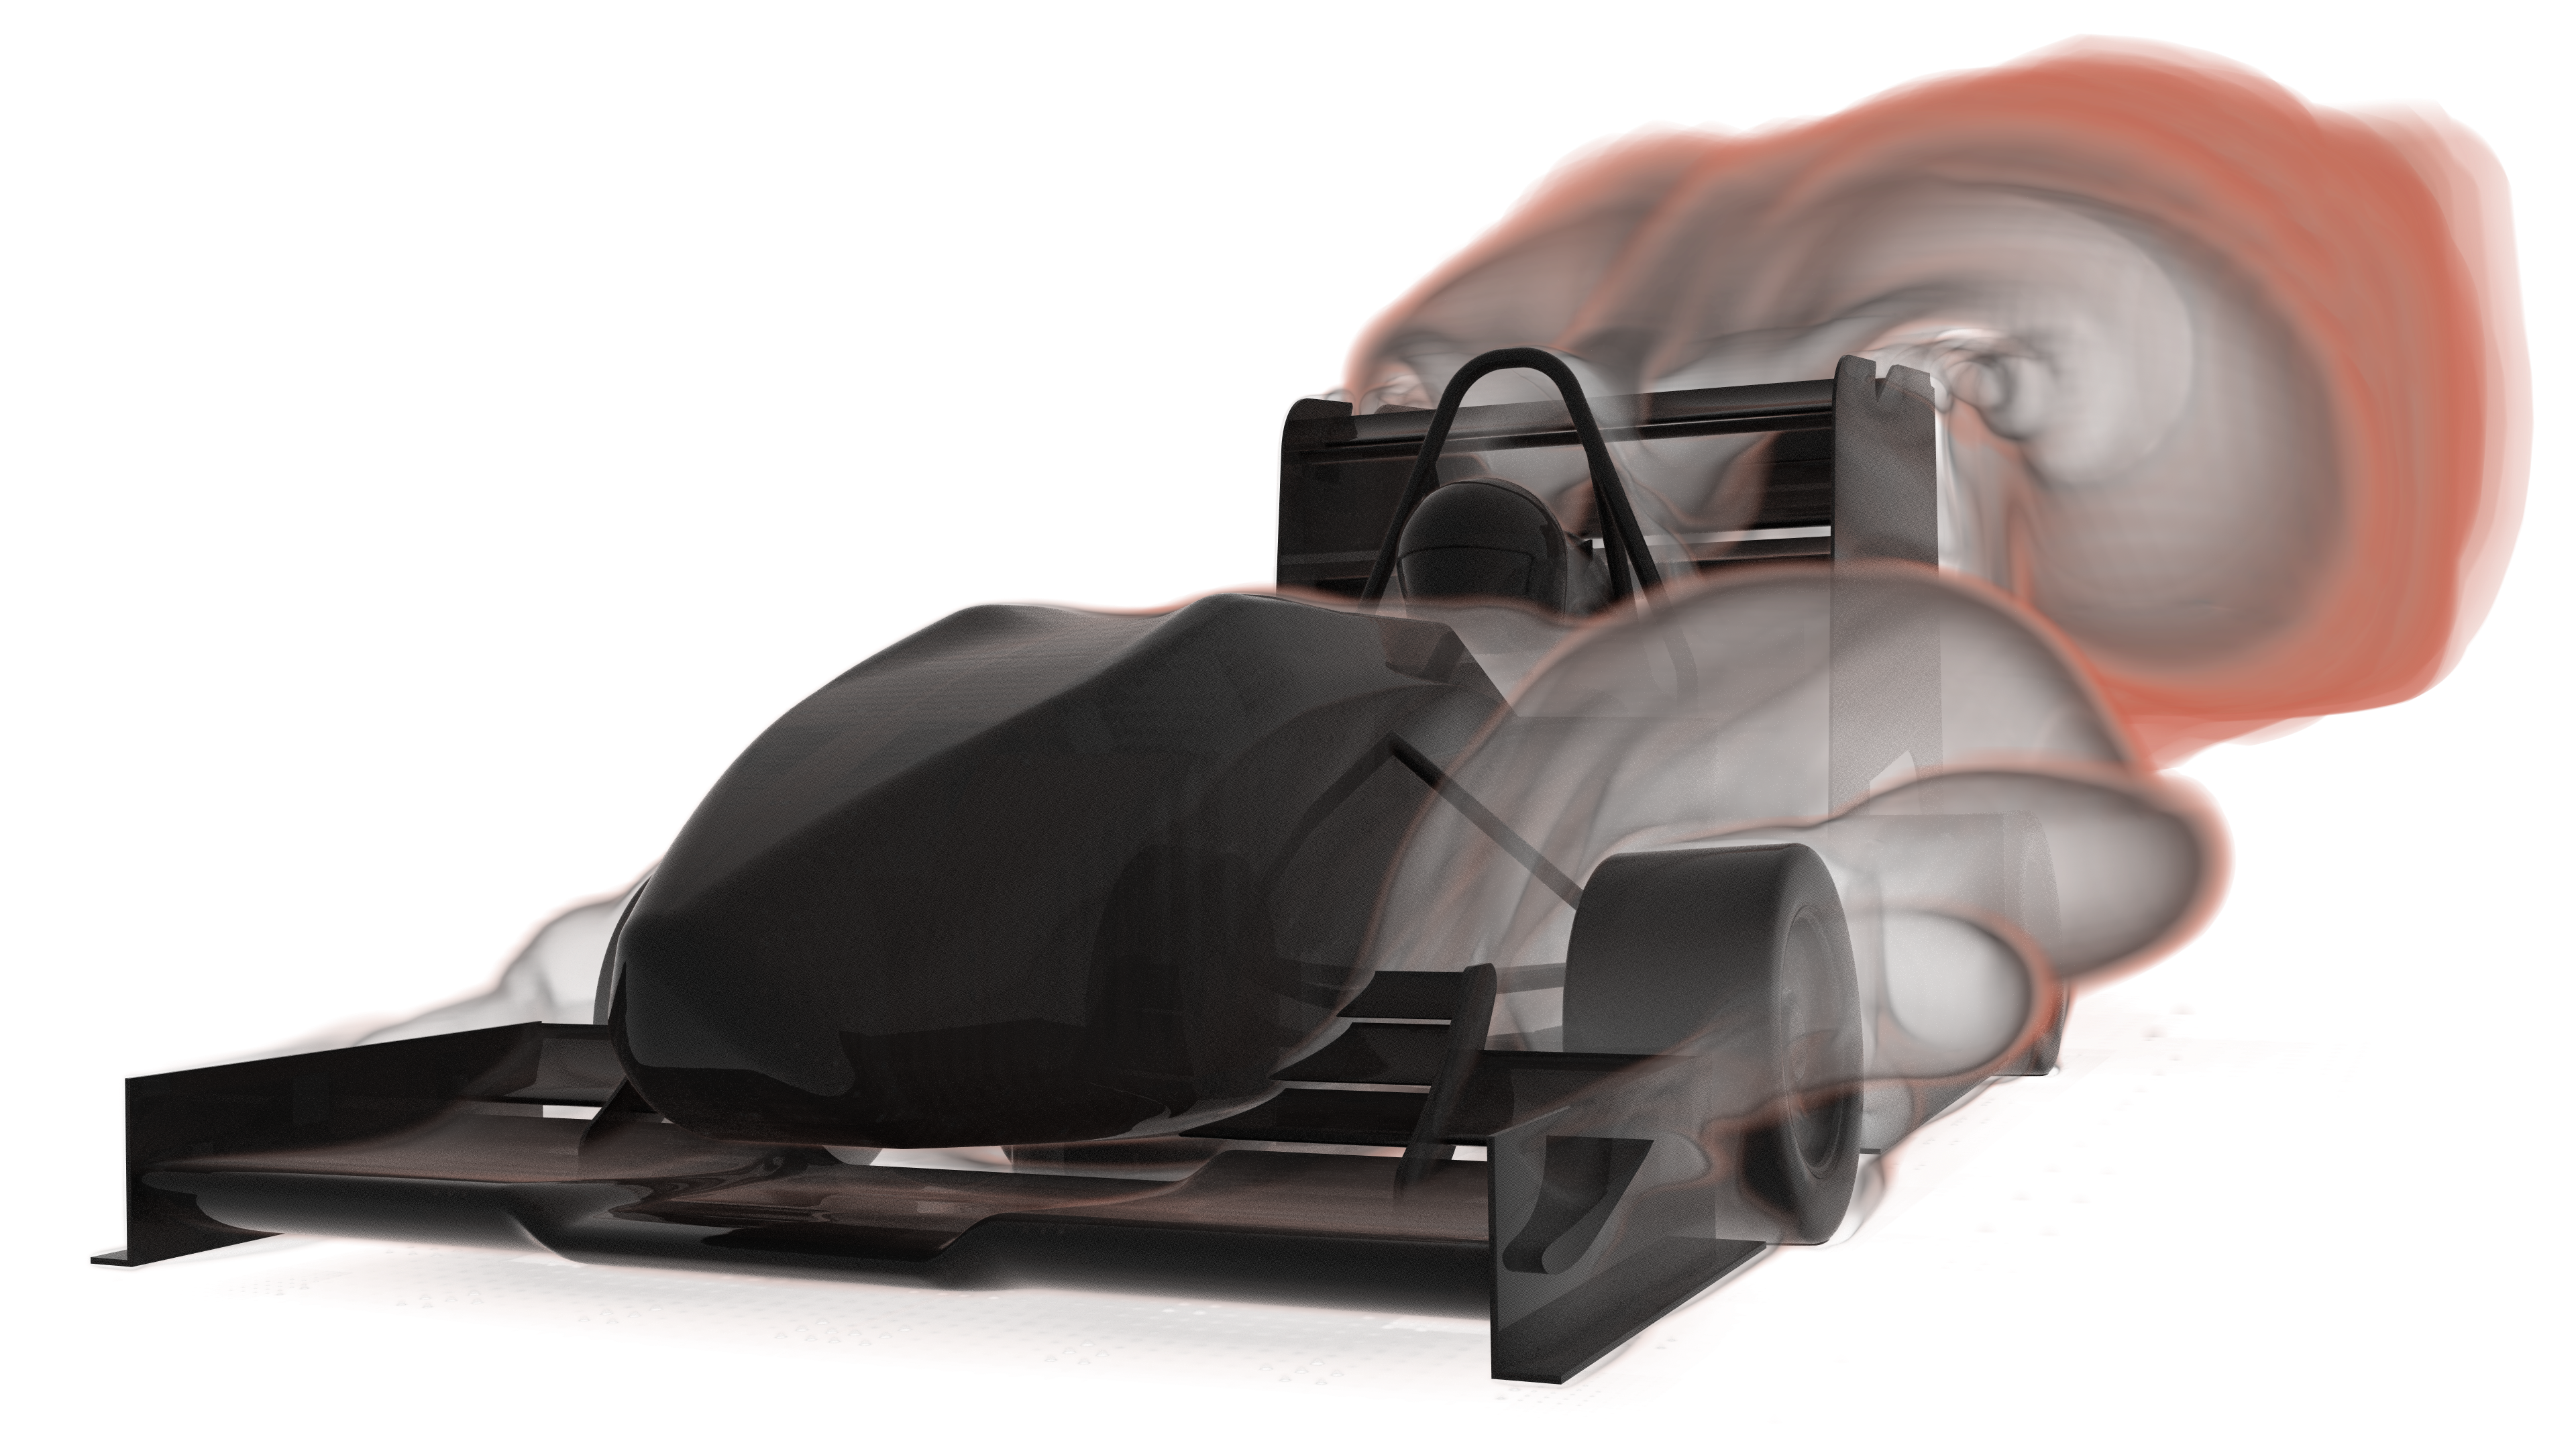
\includegraphics[width=0.9\linewidth]{pics/Titelbild.png}
        \end{figure}
        \vfill
        \normalsize
        % Tabelle angepasst: Nur noch 3 Spalten (Label, Student 1, Student 2)
        \begin{tabular}{rrr}
            \rule{0mm}{1ex}Verfasst von:   & \studentNameone & \studentNametwo \\
            \rule{0mm}{1ex}Matrikelnummer: & \hspace*{+0.5em}\studentMatnrone & \hspace*{+0.5em}\studentMatnrtwo \\
            \rule{0mm}{1ex}Studiengang:    & \studentStudiengangone & \studentStudiengangtwo \\
            \\[2em]
            \rule{0mm}{1ex}Betreuer:       & #5 & \\
            \\[1em]
            \rule{0mm}{1ex}Abgabedatum:    & #6 & \\
        \end{tabular}
    \end{center}
    \pagebreak
}
 \addbibresource{Miscellaneous/bibliography.bib}

\begin{document}

\setlength{\extrarowheight}{4pt}

\newcommand{\studierenderNameone}{Daniel Lambrecht}
\studentone{\studierenderNameone}
{0000000}
{MB 6}

\newcommand{\studierenderNametwo}{Tobias Plenk}
\studenttwo{\studierenderNametwo}
{0000000}
{MB 6}

\Titelseite{}
{1}
{Projektarbeit}
{Vorentwicklung und Simulationsbildung für die Kühlung eines Formuala Student Rennwagen}
{Prof. Dr. Wagner}
{\today}

\thispagestyle{empty}
~\pagebreak
\onehalfspacing


\thispagestyle{empty}
\chapter*{Sperrvermerk }

\bigskip
\bigskip
\bigskip


\begin{enumerate}
    \item Die vorliegende Arbeit enthält vereinsinterne Informationen und vertrauliche              Daten des Dynamics
            e.V.. Sie darf aus diesem Grunde nur zu Prüfzwecken verwendet und ohne ausdrückliche Genehmigung
            durch den Dynamics e.V. weder Dritten zugänglich gemacht, noch ganz oder in Auszüugen veröffentlicht werden. 
\item Die Sperrfrist endet 2 Jahre nach dem Einreichen der Arbeit bei der OTH Regensburg.
        Unbeschadet hiervon bleibt die Weitergabe der Arbeit an die mit der Prüfung befassten Mitarbeiter
        der Hochschule bzw. Prüufer, die ihrerseits zur Geheimhaltung verpflichtet sind, sowie die Verwendung
        der Arbeit in eventuellen prüufungsrechtlichen Rechtsschutzverfahren nach Maßgabe der geltenden verwaltungsprozessualen Regeln.
\end{enumerate}

\pagebreak
\thispagestyle{empty}
\chapter*{Eigenständigkeitserklärung }

\bigskip
\bigskip
\bigskip

\begin{enumerate}
    \item Ich bin mir darüber bewusst, dass dieses Exemplar der Projektarbeit als Teil meiner benoteten Leistung in den Besitz der OTH Regensburg übergeht.
    \item Hiermit erkläre ich, dass ich diese Projektarbeit selbst verfasst habe und sie nicht anderweitig als benotete Leistung verwendet habe. Ich habe ausschließlich die angegebenen Quellen und Werkzeuge verwendet und alle Zitate entsprechend gekennzeichnet.
\end{enumerate}

\bigskip
\bigskip
\bigskip

\hfill Regensburg, \today

\vfill
    
\line(1,0){300}
\newline
\hspace*{4em}\studierenderNameone

\bigskip
\bigskip
\bigskip
\bigskip

\line(1,0){300}
\newline
\hspace*{4em}\studierenderNametwo
\chapter*{Danksagung}
\vfill
\par Hiermit möchten wir uns zunächst bei unseren Unterstützern bedanken, ohne denen
diese Projektarbeit nicht zustande gekommen wäre. \vspace{1em}
Ein besonderer Dank geht an unseren Betreuer Herrn Prof. Dr. Andreas Wagner, der
uns mit Motivation und kritischer Betrachtung unserer Arbeit sehr geholfen und wert-
volle Hinweise gegeben hat.  \vspace{1em}
Zudem möchten wir uns auch bei unseren Teamkollegen des Dynamics e.V. bedanken.
\vspace{4em}



\chapter*{Abstract}
Testing 

\lipsum[1-3]


\pagenumbering{Roman}
\setcounter{page}{1}

\setcounter{tocdepth}{2}
\tableofcontents
\pagebreak

\listoffigures
\pagebreak

\listoftables
\pagebreak

\chapter*{Abkürzungsverzeichnis}
\begin{acronym}[KDE]
\acro{cl}[$C_L$]{Auftriebskoeffizient}
\acro{cd}[$C_D$]{Widerstandskoeffizient}
\acro{CFK}[$CFK$]{Kohlenstofffaserverstärkten Kunststoff}
\acro{CFD}[$CFD$]{Computational Fluid Dynamics}
\acro{FSG}[$FSG$]{Formula Student Germany}
\acro{CICS}[$CICS$]{ Cockpit Internal Cross Section}
\acro{IA}[$IA$]{Impact Attenuator}
\acro{RP}[$RP$]{Racing Project}
\acro{EBS}[$EBS$]{Emergency Brake System}
\acro{DV}[$DV$]{Driverless}
\acro{HVD}[$HVD$]{High Voltage Disconnect}
\acro{PSP}[$PSP$]{Projektstrukturplan}
\acro{FSAE}[$FSAE$]{Formula SAE}
\acro{AP}[$AP$]{Arbeitspaket}
\end{acronym}
\pagebreak

\renewcommand{\nomname}{Formelzeichen}
\makenomenclature
\nomenclature[$C_P$]{$C_P$}{Druckkoeffizient}
\nomenclature[$P$]{$P$}{statischer Druck [Pa]}
\nomenclature[$P_\infty$]{$P_\infty$}{Umgebungsdruck [Pa]}
\nomenclature[$\rho$]{$\rho$}{Luftdichte [\SI{}{\kilo\gram\per\meter\cubed}]}
\nomenclature[$v_\infty$]{$v_\infty$}{Simulationsgeschwindigkeit [\SI{}{\meter\per\second}]}
\nomenclature[$C_{TP}$]{$C_{TP}$}{Gesamtdruckkoeffizient}
\nomenclature[$C_L$]{$C_L$}{Abtriebskoeffizient}
\nomenclature[$C_D$]{$C_D$}{Luftwiderstandskoeffizient}
\nomenclature[$P_{dyn}$]{$P_{dyn}$}{Dynamischer Druck [Pa]}
\nomenclature[$A_{Front}$]{$A_{Front}$}{Frontale Fläche [\SI{}{\meter\squared}]}
\nomenclature[$F_Z$]{$F_Z$}{Kraft in z-Richtung [N]}
\nomenclature[$F_X$]{$F_X$}{Kraft in x-Richtung [N]}
\printnomenclature
\pagebreak

\pagenumbering{arabic}

\chapter{Einleitung}
\label{ch:einleitung}

\section{Kontext und Motivation}
\label{sec:einleitung_kontext}

Die Formula Student ist ein internationaler Konstruktionswettbewerb, bei dem Studierende innerhalb einer Saison einen Rennwagen entwickeln, fertigen und in statischen sowie dynamischen Disziplinen gegeneinander antreten lassen. Mit der Leistungsdichte elektrischer Antriebsstränge steigen die Anforderungen an das thermische Management: Elektrische Maschinen, Inverter und der Akkumulator müssen auch unter Rennbedingungen innerhalb ihrer zulässigen Temperaturgrenzen betrieben werden, ohne dass die Fahrleistung eingeschränkt wird.

Beim Dynamics e.V. hat ein unzureichendes Thermomanagement in der Vergangenheit zu erheblichen Einbußen geführt. Neben Leistungsreduzierungen (Derating) kam es zu mehreren sicherheitskritischen Ausfällen während der Fahrt. Komplette Motorausfälle durch den Übertemperaturschutz traten ebenso auf wie thermisch bedingte Schäden an Anbauteilen, darunter Felgen, Dichtungen und Lager. Die Ursachen, Auswirkungen und Konsequenzen dieser Ausfälle werden in Kapitel~\ref{ch:problemstellung} im Detail betrachtet.

Ziel dieser Projektarbeit ist die systematische Auslegung, Simulation und Validierung eines ganzheitlichen Kühlkonzepts für den Rennwagen des Dynamics e.V. Die konkreten Teilziele sind in Kapitel~\ref{ch:ziel} formuliert.

\section{Rahmenbedingungen und Abgrenzung}
\label{sec:einleitung_abgrenzung}

Die Arbeit wird durch die Rahmenbedingungen eines studentischen Rennteams geprägt. Zeit und Budget sind stark begrenzt. Die Testzeit am Fahrzeug ist knapp, und da nicht absehbar ist, wann das Gesamtfahrzeug für Messungen bereit ist, kann ein Messvorhaben unter Umständen nicht über die Vorbereitung hinauskommen. Eine zusätzliche Instandhaltung des Fahrzeugs durch die Verfasser ist aus Kapazitätsgründen nicht möglich. Hinzu kommt eine lückenhafte Datenlage: Für viele Komponenten liegen keine belastbaren Wirkungsgradkennfelder vor, sodass Kennwerte erst durch Versuche am Motorprüfstand ermittelt oder durch Herstellerangaben ersetzt werden müssen.

Daraus ergibt sich der Schwerpunkt der Arbeit. Im Mittelpunkt stehen die Erarbeitung von Messtechnik und Messvorgehen, die Analyse der bestehenden Kühlsysteme und angrenzenden Systeme sowie die Modellierung der Verlustleistungen der relevanten Komponenten. Auf dieser Basis wird eine erste Auslegung vorgenommen. Die Arbeit versteht sich zugleich als Grundlage für künftige Entwicklungen, in denen die vereinfachten Modelle, etwa das hier entwickelte Akkumodell, durch genauere ersetzt werden können.

Folgende Punkte sind nicht Ziel der Arbeit:
\begin{itemize}
    \item Der Aufbau eines perfekten Akku-, Motor- oder Wechselrichtermodells. Die Modelltiefe beschränkt sich auf die Grundlagen, die später erweitert werden können.
    \item Die Neuentwicklung einzelner Komponenten, etwa eines eigenen Radiators oder Lüfters für den Anwendungsfall. Dimensionierung und Integration in das bestehende Fahrzeug sind dagegen Teil der Arbeit.
    \item Eine Neuentwicklung der Motorenkühlung. Aus Budgetgründen ist eine Neubeschaffung innerhalb der nächsten Saison nicht möglich. Stattdessen werden Modellierungsansätze und konkrete Verbesserungsmöglichkeiten erarbeitet, die in die künftige Motorauslegung einfließen können.
\end{itemize}

Nicht alle Komponenten konnten von den Verfassern allein aufgebaut werden. Vor allem im Bereich Elektrotechnik und Mechatronik wurden andere Subteams des Dynamics e.V. hinzugezogen, mit der Entwicklung beauftragt oder in Kooperation beteiligt. Im Mechanischen wurden die erforderlichen Arbeiten selbst ausgeführt, auch dort, wo sie nur mittelbaren Bezug zu dieser Arbeit hatten. Im weiteren Verlauf wird jeweils kenntlich gemacht, wo auf bestehende Strukturen verwiesen wird, wo andere Subteams unterstützt haben und wo Entwicklungen extern stattgefunden haben.

\section{Aufbau der Arbeit}
\label{sec:einleitung_aufbau}

Die Arbeit gliedert sich wie folgt: Kapitel~\ref{ch:ziel} beschreibt das Ziel der Arbeit, Kapitel~\ref{ch:problemstellung} definiert die Problemstellung mit den aufgetretenen Ausfällen, ihren Ursachen und Konsequenzen. Kapitel~\ref{ch:messtechnik} stellt die Messtechnik und die Systemarchitektur vor. Darauf aufbauend behandelt Kapitel~\ref{ch:testplanung} die Testplanung mit den Grundlagen, Anforderungen und dem relevanten Regelwerk. Kapitel~\ref{ch:systemmodelle} beschreibt die Systemmodelle für Akku und Motoren sowie das Thermonetzwerk. In Kapitel~\ref{ch:messungen} wird die Durchführung der Messungen am Motorprüfstand dokumentiert. Kapitel~\ref{ch:konstruktion} begründet die Konstruktionsentscheidungen für die Integration ins Fahrzeug. Kapitel~\ref{ch:fazit} fasst die Ergebnisse zusammen und gibt einen Ausblick auf künftige Arbeiten.
\chapter{Ziel der Arbeit}
\label{ch:ziel}

Das Ziel dieser Arbeit ist die Vorentwicklung eines Kühlkonzepts für den Formula Student Rennwagen des Dynamics e.V. und der Aufbau der Simulationsgrundlagen, mit denen dieses Konzept bewertet und künftig weiterentwickelt werden kann. Ausgangspunkt ist die in Kapitel~\ref{ch:problemstellung} beschriebene Problemstellung: Die Komponenten sollen auch unter Rennbedingungen innerhalb ihrer Temperaturgrenzen betrieben werden, ohne dass Leistung reduziert werden muss oder Komponenten ausfallen.

Daraus leiten sich folgende Teilziele ab:

\begin{enumerate}
    \item \textbf{Analyse des Ist-Zustands:} Die aufgetretenen Ausfälle werden hinsichtlich Ursachen und Konsequenzen eingeordnet. Die bestehenden Kühlkreisläufe werden hydraulisch charakterisiert, indem Widerstandswerte von Schlauch, Motor, Radiator und Inverter am Fahrzeug bestimmt werden.

    \item \textbf{Messtechnik und Messvorgehen:} Die Sensorik für Volumenstrom, Temperatur und Differenzdruck wird ausgelegt, im Labor validiert und in die Systemarchitektur integriert. Für Motorprüfstand und Fahrzeug wird ein Testplan erarbeitet, der Messpunkte, Fahrmanöver und Randbedingungen festlegt.

    \item \textbf{Charakterisierung der Akkuzellen:} Durch Lade- und Entladeversuche sowie eine thermische Vermessung werden Kennwerte der Akkuzellen ermittelt, die als Grundlage für das Akku-Verlustleistungsmodell dienen.

    \item \textbf{Modellbildung:} Für die relevanten Komponenten (Motoren, Inverter, Akku) werden Verlustleistungs- und Wärmemodelle aufgebaut und in einem modularen Systemmodell in \textit{Matlab/Simulink} zusammengeführt. Dieses ermöglicht den Vergleich verschiedener Kreislaufarchitekturen, etwa serieller und paralleler Durchströmung. Die Modelltiefe ist bewusst begrenzt, damit die Modelle später erweitert werden können, etwa um genauere Akku- oder Motormodelle.

    \item \textbf{Strömungsanalyse:} Mittels CFD werden Kühlgeometrien untersucht, um lokale Hotspots zu identifizieren und Verbesserungspotenzial aufzuzeigen. % PRÜFEN: Umfang und Komponenten der CFD

    \item \textbf{Auslegung und Integration:} Radiator, Lüfter, Pumpen und Kreislauflayout werden dimensioniert und unter Berücksichtigung von Aerodynamik, Package und Wartbarkeit in das Fahrzeug integriert. Das Entlüftungskonzept wird überarbeitet, um den Aufwand bei Events zu verringern.

    \item \textbf{Messungen am Motorprüfstand und Ausblick:} Die Messungen am Motorprüfstand werden vorbereitet und soweit möglich durchgeführt. Auf Basis der Ergebnisse werden Verbesserungsmöglichkeiten für künftige Fahrzeuggenerationen abgeleitet, insbesondere für die Motorenkühlung.
\end{enumerate}

Die Arbeit verfolgt dabei einen kombinierten Ansatz aus Simulation und experimenteller Absicherung. Nicht Teil der Arbeit sind eine vollständige Validierung der Modelle, eine Sensitivitätsanalyse sowie detaillierte elektromagnetische Motormodelle (z.\,B. mit \textit{ANSYS Maxwell}); sie werden im Ausblick (Kapitel~\ref{ch:fazit}) aufgegriffen. Die Abgrenzung ist in Abschnitt~\ref{sec:einleitung_abgrenzung} beschrieben.
\chapter{Definition der Problemstellung}
\label{ch:problemstellung}

Die thermische Auslegung des Kühlkreislaufs stellt bei der Entwicklung eines Formula Student Fahrzeugs eine der kritischsten Herausforderungen dar. Die aktuelle Problematik lässt sich in zwei Hauptbereiche unterteilen: eine unzureichende empirische Datenbasis sowie eine nachweislich unterdimensionierte Kühlkapazität unter Wettbewerbsbedingungen.

\section{Mangelnde Informationsgrundlage}
\label{sec:informationsgrundlage}

Ein fundamentales Hindernis bei der Dimensionierung des Kühlsystems ist die fehlende Datenbasis zur Bestimmung der thermischen Lasten.

\begin{itemize}
    \item \textbf{Verlustleistungsbestimmung:} Es liegen keine validierten Modelle oder Messreihen vor, um die Verlustleistung der Hauptkomponenten -- Akkumulator, Inverter und Elektromotoren -- über einen gesamten Fahrzyklus zu quantifizieren. Dies ist die grundlegende Ursache aller nachgelagerten Dimensionierungsprobleme.
    \item \textbf{Dimensionierungsrisiko:} Ohne die Kenntnis der tatsächlichen Wärmeströme basiert die Auslegung der Radiatoren und Pumpenleistungen auf Schätzungen. Dies führt entweder zu Mehrgewicht durch Überdimensionierung oder -- wie im vorliegenden Fall -- zu thermischer Überlastung im Betrieb.
    \item \textbf{Lückenhaftes Sensornetz:} Die aktuell erfassten Messgrößen beschränken sich im Wesentlichen auf Komponententemperaturen. Entscheidende Größen wie der Volumenstrom im Kühlkreislauf werden nicht gemessen, wodurch eine vollständige Systemanalyse nicht möglich ist. Dass Felgenbetten durch Infrarotstrahlung der Bremsscheiben schmolzen, ohne dass ein Sensor in diesem Bereich vorhanden war, verdeutlicht diese Lücke exemplarisch.
    \item \textbf{Fehlende thermische Simulation:} Aktuell wird das Kühlsystem gebaut und anschließend im Fahrbetrieb erprobt. Eine vorgelagerte Simulation -- etwa auf Basis eines Lumped-Parameter-Modells -- würde kostspielige Iterationen am realen Fahrzeug reduzieren und eine gezieltere Auslegung ermöglichen.
\end{itemize}

Die folgenden Messdaten illustrieren die Konsequenzen dieser Datenlücken im realen Wettbewerbsbetrieb.

\section{Analyse der thermischen Unterdimensionierung}
\label{sec:thermische_analyse}

Die Auswertung der Telemetriedaten vergangener Testtage und Wettbewerbe verdeutlicht die Defizite des aktuellen Systems. Während Teilsysteme wie der Inverter und der Akkumulator innerhalb der spezifizierten Betriebsgrenzen verbleiben, zeigen die Antriebseinheiten ein kritisches thermisches Verhalten.

\subsection{Vergleich: Testbetrieb vs. Wettbewerbslast}

\paragraph{Testtag (Vorbereitung FSG):}
\begin{figure}[H]
    \centering
    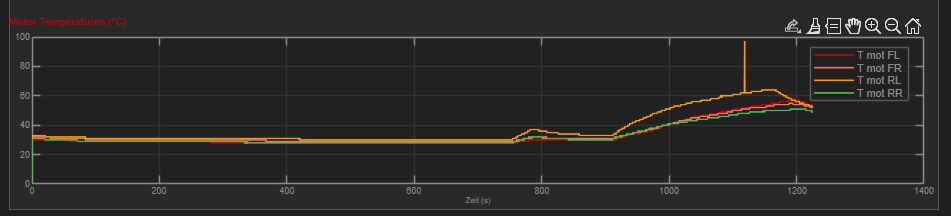
\includegraphics[width=1.0\textwidth]{pics/1.Testtage.jpeg}
    \caption{Temperaturverlauf während der Testphase: Der Motor \textit{Rear Left} (gelbe Kurve) zeigt eine überproportionale Erwärmung gegenüber den übrigen Antriebseinheiten bei moderater Last.}
    \label{fig:log_testtag}
\end{figure}

In dieser Phase zeigten sich erste Auffälligkeiten. Der hintere linke Motor (\textit{Rear Left}) wies eine deutlich höhere Temperaturzunahme auf als die übrigen Motoren. Die Inverter-Temperaturen verharrten auf einem unkritischen Niveau, was auf Potential zur Reduktion der Kühlleistung in diesem Zweig hindeutet. Die Zelltemperaturen des Akkumulators verliefen homogen und innerhalb der Zielparameter.

\paragraph{Endurance FSG:}
\begin{figure}[H]
    \centering
    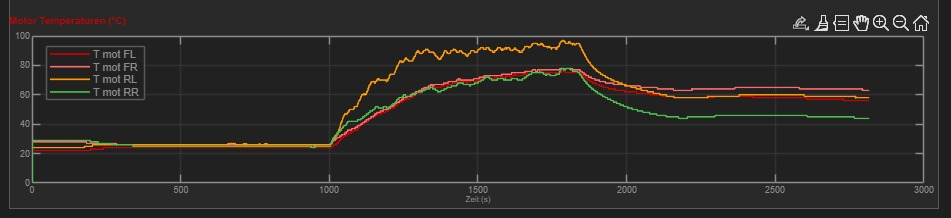
\includegraphics[width=1.0\textwidth]{pics/FSG_Endu_mit_Derating.jpeg}
    \caption{Telemetrie-Log FSG Endurance: Der \textit{Rear Left} Motor erreicht die De-Rating-Schwelle von $90\,^\circ\text{C}$, woraufhin das Managementsystem die Systemleistung automatisch begrenzt.}
    \label{fig:log_fsg_derating}
\end{figure}

Unter Wettbewerbsbedingungen verschärfte sich die Situation deutlich. Während die Frontmotoren und der hintere rechte Motor unterhalb der De-Rating-Grenze von $90\,^\circ\text{C}$ blieben, stagnierte der Motor \textit{Rear Left} bei ca. $100\,^\circ\text{C}$. Das Managementsystem griff daraufhin automatisch ein und drosselte die elektrische Leistung zum Schutz der Hardware, was einen messbaren Performanceverlust zur Folge hatte.

\paragraph{Endurance FS ATA:}
\begin{figure}[H]
    \centering
    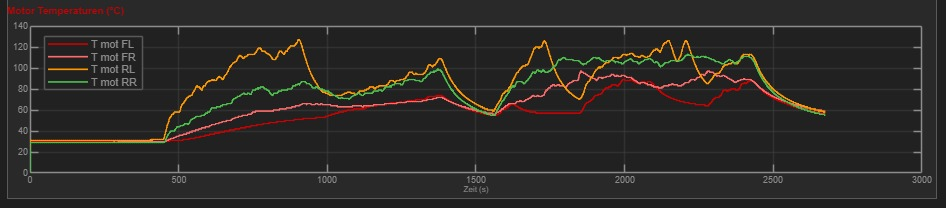
\includegraphics[width=1.0\textwidth]{pics/FSATA_Endu_mit_Abschlatung.jpeg}
    \caption{Thermische Grenzbelastung im FS ATA Endurance: Nach Deaktivierung des De-Ratings kam es bei Temperaturen über $120\,^\circ\text{C}$ zu insgesamt fünf Notabschaltungen (\textit{Engine-Cutoffs}).}
    \label{fig:log_ata_cutoffs}
\end{figure}

Um die Leistungsdrosselung zu umgehen, wurde das De-Rating für den Wettbewerb in Italien deaktiviert. Der Hardwareschutz erfolgte damit ausschließlich durch Notabschaltung. Infolgedessen kam es während des Rennens zu fünf temperaturbedingten Abschaltungen, die den Rennverlauf erheblich beeinträchtigten.

\subsection{Asymmetrisches Thermoverhalten der Antriebseinheiten}
\label{subsec:asymmetrie}

Ein bisher ungeklärter Befund ist das konsistent abweichende Temperaturverhalten des Motors \textit{Rear Left}. Dieser überschreitet in nahezu allen aufgezeichneten Betriebssituationen als erster die kritischen Schwellwerte, während die übrigen drei Motoren deutlich kühler bleiben. Mögliche Ursachen liegen in einer ungleichmäßigen Durchflussverteilung im Kühlkreislauf, in der geometrischen Anordnung der Kühlanbindung oder in einer mechanischen Ursache, die zu erhöhter lokaler Verlustleistung führt. Dieser Befund ist bislang nicht systematisch untersucht worden und stellt einen eigenständigen Analyseschwerpunkt dieser Arbeit dar.

\subsection{Kritische thermische Wechselwirkungen mit der Bremsanlage}
\label{subsec:bremse}

\begin{figure}[htbp]
    \centering
    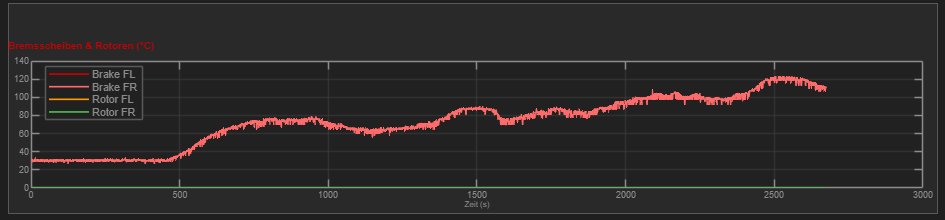
\includegraphics[width=0.9\textwidth]{pics/Brake_Temp_FS_ATA.PNG}
    \caption{Thermische Belastung der Bremsperipherie: Der Anstieg der Rotortemperatur auf über $100\,^\circ\text{C}$ korreliert zeitlich mit den gemeldeten Fading-Effekten und der Infrarot-Abstrahlung auf das Felgenbett.}
    \label{fig:brems_log_ata}
\end{figure}

Zusätzlich zur thermischen Belastung der Antriebskomponenten wurde die Bremsanlage als weiterer kritischer Wärmeeintrag identifiziert:

\begin{itemize}
    \item \textbf{Bremsversagen (Fading):} Temperaturen von über $100\,^\circ\text{C}$ an der Bremsperipherie führten zu einem deutlichen Nachlassen der Bremswirkung und beeinträchtigten die Fahrsicherheit.
    \item \textbf{Strukturelles Versagen durch Strahlungswärme:} In der Saison 2024 führte die Infrarotstrahlung der Bremsscheiben zum Schmelzen der Felgenbetten -- ein Schadensfall, der durch geeignete Messtechnik und thermische Schutzmaßnahmen hätte verhindert werden können.
\end{itemize}

\section{Gewicht-Kühlleistung-Zielkonflikt}
\label{sec:tradeoff}

Die Dimensionierung des Kühlsystems unterliegt einem grundlegenden Zielkonflikt: Größere Radiatoren und leistungsstärkere Pumpen verbessern die Wärmeabfuhr, erhöhen jedoch Gewicht und aerodynamischen Widerstand -- beides kritische Größen im Formula Student Kontext. Ohne ein quantitatives Modell der tatsächlich abzuführenden Wärmemengen kann dieser Trade-off nicht rational bewertet werden. Die bisherige Auslegung basierte auf Erfahrungswerten, was die beschriebenen Probleme begünstigt hat.

\section{Auslegungspunkt und Umgebungsbedingungen}
\label{sec:auslegungspunkt}

Ein weiterer ungeklärter Aspekt betrifft den thermischen Auslegungspunkt des Gesamtsystems. Die Wettbewerbe finden unter unterschiedlichen klimatischen Bedingungen statt: Die FSG in Deutschland und die FS ATA in Italien unterscheiden sich sowohl in Umgebungstemperatur als auch in Luftfeuchtigkeit erheblich. Es ist aktuell nicht definiert, für welche Umgebungsbedingungen das Kühlsystem ausgelegt ist und ob die gewählte Auslegung die ungünstigsten zu erwartenden Bedingungen abdeckt. Dies erschwert eine belastbare Bewertung der Systemreserven.

\section{Historische Analyse der Endurance-Zuverlässigkeit}
\label{sec:historie}

Um die Relevanz einer verbesserten Kühlungsstrategie zu verdeutlichen, fasst Tabelle~\ref{tab:endurance_historie} die Ergebnisse der vergangenen Endurance-Läufe sowie die jeweiligen Hauptursachen für Ausfälle oder Leistungseinschränkungen zusammen.

\begin{table}[htbp]
    \centering
    \caption{Analyse der Endurance-Ergebnisse von 2021 bis 2025}
    \label{tab:endurance_historie}
    \small
    \renewcommand{\arraystretch}{1.25}
    \begin{tabularx}{\textwidth}{|l|l|l|X|}
        \hline
        \textbf{Jahr} & \textbf{Event} & \textbf{Status} & \textbf{Primäre Ausfallursache / Problem} \\
        \hline\hline
        2021 & FSG    & DNF    & Elektrische Defekte (LV-Platine) \\
        2022 & FSG    & DNS    & Defekt im Akkumulator-Container \\
        2023 & FSG    & DNS    & Mechanisches Versagen (Radaufhängung) \\
        2023 & FSAA   & DNF    & Mechanisches Versagen (Radaufhängung) \\
        \hline
        2024 & FSCZ   & DNF    & \textbf{Thermische Überlastung der Bremse} \\
        2024 & FSG    & DNF    & \textbf{Schmelzende Felgenbetten durch Strahlungshitze} \\
        2024 & FS ATA & Erfolg & Erster erfolgreicher AWD-Endurance \\
        \hline
        2025 & FS CZ  & DNS    & Mechanisches Versagen (Radaufhängung) \\
        2025 & FS G   & DNF    & \textbf{Dichtungsschaden infolge von Überhitzung} \\
        2025 & FS ATA & Erfolg & Zielankunft mit \textbf{5 Engine-Cutoffs} und massiver Leistungsbegrenzung \\
        \hline
    \end{tabularx}
\end{table}

\noindent\small{DNF = Did Not Finish, DNS = Did Not Start}
\vspace{1em}

\subsection{Identifikation des thermischen Bottlenecks}
\label{subsec:bottleneck}

Die Auswertung der vergangenen fünf Jahre zeigt eine deutliche Verschiebung der technischen Herausforderungen. Während in der frühen Phase von 2021 bis 2023 primär grundlegende elektrische und mechanische Zuverlässigkeit im Vordergrund stand, hat sich seit der Einführung des Allradantriebs die thermische Standfestigkeit als kritischer Limitierungsfaktor etabliert.

Besonders die Saisons 2024 und 2025 verdeutlichen, dass das Fahrzeug mechanisch und elektrisch konkurrenzfähig ist, jedoch durch unzureichende Wärmeabfuhr am Erreichen der Ziellinie gehindert wird. Das Schmelzen von Felgenbetten (FSG 2024) sowie thermisch bedingte Dichtungsschäden (FSG 2025) sind klare Indikatoren dafür, dass das thermische System die Grenzen der Betriebssicherheit erreicht hat. Die vorliegende Arbeit setzt genau an diesem Punkt an und zielt darauf ab, die beschriebenen Defizite systematisch zu erfassen und eine fundierte Grundlage für die Auslegung eines verbesserten Kühlsystems zu schaffen.
\section{Benchmark-Analyse: Kühlsysteme der FS-Teams 2025}

Im Rahmen der Konzeptentwicklung wurde eine Benchmark-Analyse der Engineering Design Reports (EDR) führender Teams durchgeführt. Dabei zeigten sich zwei grundlegend verschiedene Strategien: die konventionelle Wasserkühlung für hohe Leistungsdichte und die innovative Luftkühlung zur Gewichtsoptimierung.

\begin{table}[h]
    \centering
    \caption{Vergleich der Kühlkonzepte ausgewählter Teams (Saison 2025)}
    \label{tab:kuehlung_benchmark}
    \begin{tabular}{l|p{4cm}|p{4cm}|p{3.5cm}}
        \hline
        \textbf{Team} & \textbf{Kühlung Antrieb} & \textbf{Kühlung Akkumulator} & \textbf{Besonderheiten} \\ \hline
        \textbf{Schanzer Racing} & \textbf{Wassergekühlt}: 2 Kreisläufe, 4 Radiatoren in den Sidepods & \textbf{Luftgekühlt}: Optimierte Sidepod-Einlässe & Kühlung von 4 Motoren + 2 Dual-Invertern \\ \hline
        \textbf{Joanneum Racing} & \textbf{Luftgekühlt}: Aktive Lüfter ziehen Luft durch Uprights & \textit{Nicht explizit spezifiziert} & Verzicht auf Pumpen/Radiatoren spart Gewicht \\ \hline
        \textbf{Ecurie Aix}      & Fokus auf Verlustminimierung im Inverter/Motor & \textbf{Optimiertes Thermomanagement} & Fokus auf Redesign zur Effizienzsteigerung \\ \hline
        \textbf{AMZ Racing}      & Hydraulische Elemente in Sidepods integriert & \textit{Keine Detailangabe} & Fokus auf Packaging in den Sidepods \\ \hline
        \textbf{Strohm + Söhne}  & AMK FSE Kit Standardkühlung & Fokus auf Rekuperations-Management & Effizienz durch Energiemanagement \\ \hline
    \end{tabular}
\end{table}

\subsection{Detaillierte Betrachtung der Konzepte}

\subsubsection{Aktive Luftkühlung (Beispiel: Joanneum Racing Graz)}
Ein interessanter Ansatz findet sich beim JR25 von Joanneum Racing. Das Team setzt auf eine reine Luftkühlung der Radnabenmotoren. Hierbei sind Kühlrippen direkt in die Uprights integriert, und elektrische Lüfter sorgen für einen konstanten Luftstrom. Der primäre Vorteil liegt in der Reduktion der Systemkomplexität: Da keine Wasserpumpen, Schläuche oder Ausgleichsbehälter benötigt werden, sinkt das Fahrzeuggewicht und das Risiko für Leckagen während des Endurance-Wettbewerbs wird eliminiert.

\subsubsection{Zwei-Kreis-Wasserkühlung (Beispiel: Schanzer Racing Electric)}
Das Team Schanzer Racing (SRe25) verfolgt hingegen ein klassisches Hochleistungskonzept. Um die thermische Last der vier Motoren und der zwei Dual-Inverter (platziert im Front- und Heckbereich) abzuführen, werden zwei separate Wasserkreisläufe verwendet. Die Wärmeabfuhr erfolgt über vier Radiatoren, die in den aerodynamisch optimierten Sidepods untergebracht sind. Dieses System ermöglicht eine stabilere Temperaturführung bei hohen Umgebungstemperaturen, erkauft dies jedoch durch ein höheres Systemgewicht.

\subsubsection{Thermomanagement im Akkumulator (Beispiel: Ecurie Aix)}
Ecurie Aix legt beim eax04 den Schwerpunkt auf die thermische Optimierung des Akkumulators. Durch ein Redesign der Zellkontaktierung und des internen Aufbaus sollen ohmsche Verluste minimiert werden, was die thermische Last von vornherein reduziert. Ziel ist es, die Betriebstemperatur der Zellen auch ohne massiven Kühlaufwand im optimalen Fenster zu halten.
\chapter{Messtechnik und Systemarchitektur}
\label{ch:messtechnik}

Um eine fundierte Analyse des Kühlsystems durchzuführen und die theoretischen Modelle zu validieren, ist eine präzise und hochfrequente Datenerfassung unerlässlich. Dieses Kapitel beschreibt die messtechnische Infrastruktur des Fahrzeugs sowie die zugrunde liegende Systemarchitektur. Dabei wird zunächst auf die bereits im Fahrzeug integrierte Bestandssensorik eingegangen, bevor die im Rahmen dieser Arbeit implementierten Erweiterungen zur detaillierten thermischen Überwachung erläutert werden. Ziel ist es, eine lückenlose Messkette abzubilden – von der physikalischen Messgröße über die Signalaufbereitung bis hin zur digitalen Protokollierung im Datenlogger.

\section{Bestandssensorik und Infrastruktur}
\label{sec:bestandssensorik}

Die am Fahrzeug vorhandene elektronische Infrastruktur bildet das Rückgrat der Datenerfassung und Steuerung, auf dem die thermische Analyse dieser Arbeit aufbaut. Ein tiefgreifendes Verständnis der vorhandenen Signalwege ist essenziell, um die Qualität und Aussagekraft der geloggten Daten korrekt einordnen zu können.

\begin{figure}[htbp]
    \centering
    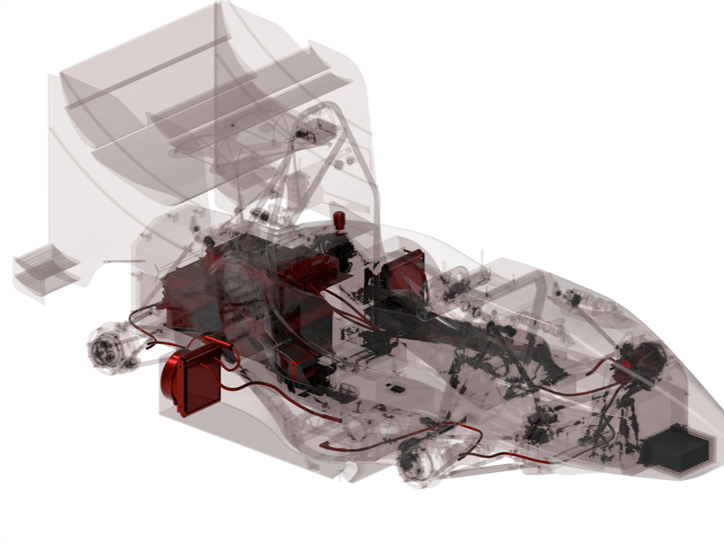
\includegraphics[width=0.9\textwidth]{pics/Systemarchtiektur_RP25e.png}
    \caption{Schematische Übersicht der fahrzeugseitigen Systemarchitektur: Signalfluss von den Sensoren über VCU und PDU bis zum Datenlogger.}
    \label{fig:Systemarchtiektur_RP25e}
\end{figure}

\subsection{Zentrale Steuereinheiten (VCU \& PDU)}
\label{subsec:vcu_pdu}

Die Steuerung und Energieversorgung des Fahrzeugs wird durch zwei zentrale Einheiten realisiert, die maßgeblich an der Datenerhebung für das Kühlsystem beteiligt sind.

\paragraph{Vehicle Control Unit (VCU)}
Die VCU stellt das Herzstück der Fahrzeugsteuerung dar. Auf ihr wird die Steuerungssoftware ausgeführt, welche die gesamte Betriebsstrategie verwaltet. Im Kontext des Kühlsystems übernimmt die VCU zwei Hauptaufgaben:
\begin{enumerate}
    \item \textbf{Aktorik-Ansteuerung:} Basierend auf definierten Temperaturschwellwerten regelt die VCU die Drehzahl der Kühlmittelpumpen und die Aktivierung der Lüfter über ein PWM-Signal.
    \item \textbf{Daten-Gateway:} Sie fungiert als zentraler Knotenpunkt, der Messwerte der Inverter via CAN-Bus sowie analoge Sensordaten empfängt, verarbeitet und an den Datenlogger weiterleitet.
\end{enumerate}

Eine Limitierung der VCU besteht darin, dass viele physikalische Sensoren aufgrund geringer Signalstärken oder hoher Ausgangsimpedanzen nicht direkt angeschlossen werden können. Diese erfordern eine vorgeschaltete Signalaufbereitung, was die Anzahl der direkt nutzbaren Sensoreingänge effektiv begrenzt.

\begin{figure}[htbp]
    \centering
    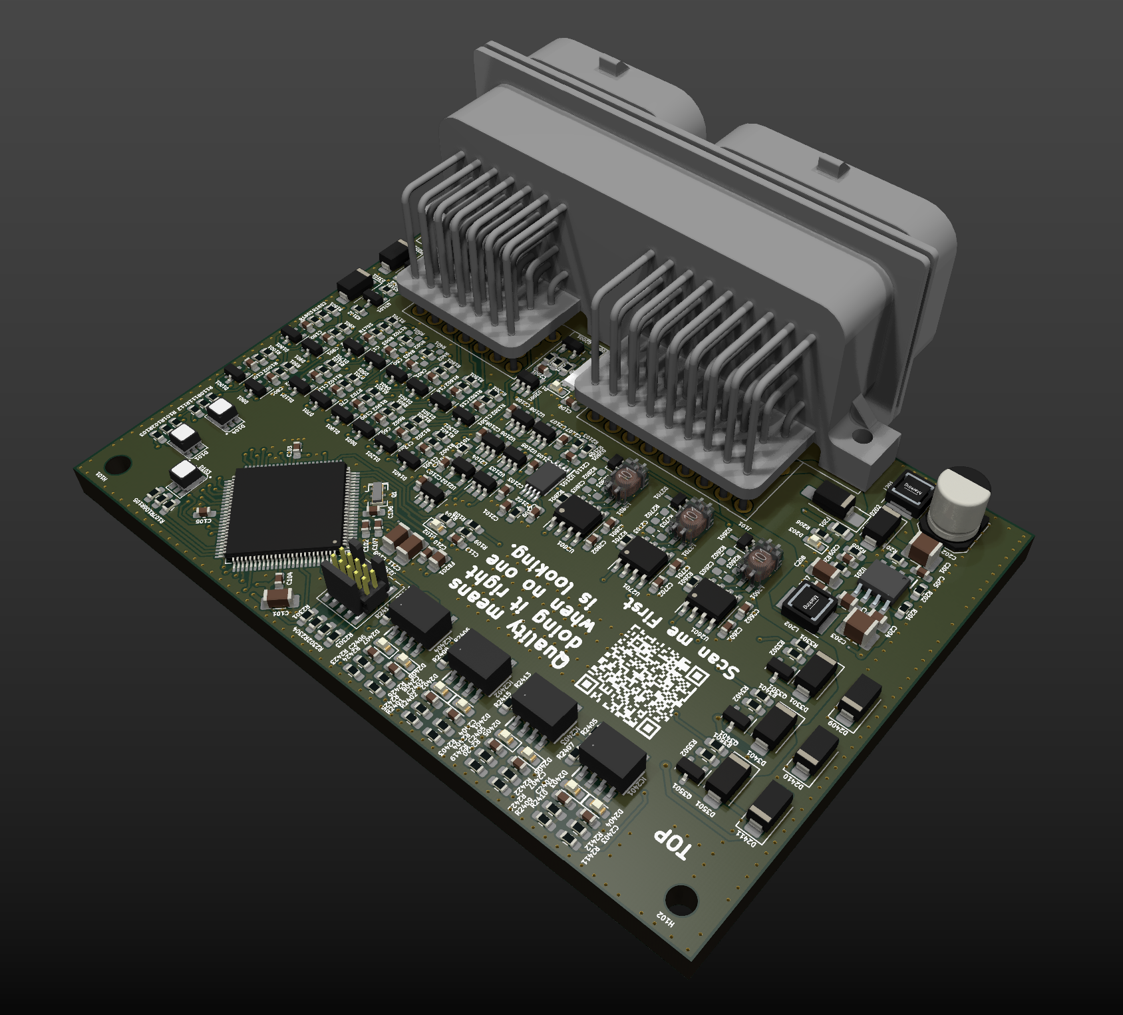
\includegraphics[width=0.7\textwidth]{pics/VCU_PCB.png}
    \caption{Übersicht der VCU}
    \label{fig:vcu_uebersicht}
\end{figure}


\paragraph{Power Distribution Unit (PDU)}
Die PDU fungiert als intelligente, softwarebasierte Stromverteilung und ersetzt klassische Schmelzsicherungen durch elektronisch überwachte Kanäle. Ihre Relevanz für die Messtechnik liegt in der kontinuierlichen Stromüberwachung der angeschlossenen Aktoren:
\begin{itemize}
    \item \textbf{Lastüberwachung:} Die PDU misst die Stromaufnahme der Kühlmittelpumpen und Lüfter. Diese Daten erlauben Rückschlüsse auf den Betriebszustand der Aktorik, beispielsweise bei Blockaden oder Trockenlauf.
    \item \textbf{Versorgungsstabilität:} Durch das Monitoring der Bordnetzspannung wird sichergestellt, dass die Sensorik stets innerhalb ihrer spezifizierten Versorgungsspannung arbeitet, was die Validität der Messergebnisse absichert.
\end{itemize}

\begin{figure}[htbp]
    \centering
    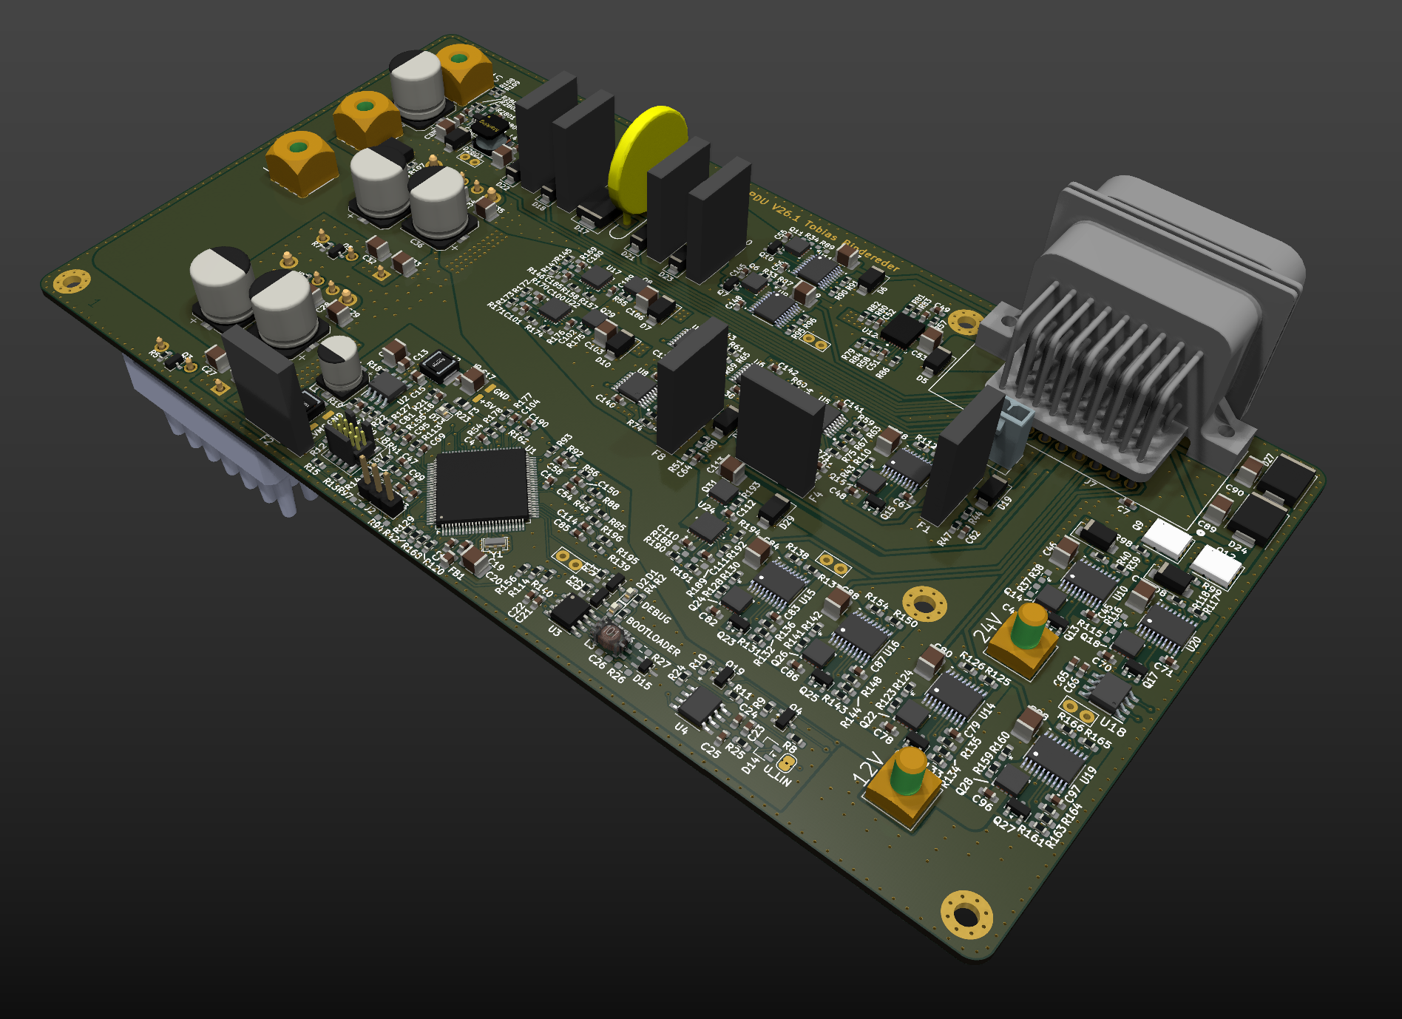
\includegraphics[width=0.7\textwidth]{pics/PDU_PCB.png}
    \caption{Übersicht der PDU}
    \label{fig:PDU_uebersicht}
\end{figure}

Zusammen bilden VCU und PDU die Grundlage, um nicht nur Temperaturen, sondern auch die dafür aufgewendete elektrische Energie und den Betriebszustand der Aktoren zu protokollieren.

\subsection{Datenerfassung und Telemetrie}
\label{subsec:datenlogger}

Die zentrale Einheit zur persistenten Speicherung aller fahrzeugrelevanten Daten ist der Datenlogger. Er erfasst kontinuierlich die von der VCU sowie den Invertern via CAN-Bus bereitgestellten Messwerte und speichert diese mit hoher Abtastrate auf einem internen Speichermedium.

\begin{figure}[htbp]
    \centering
    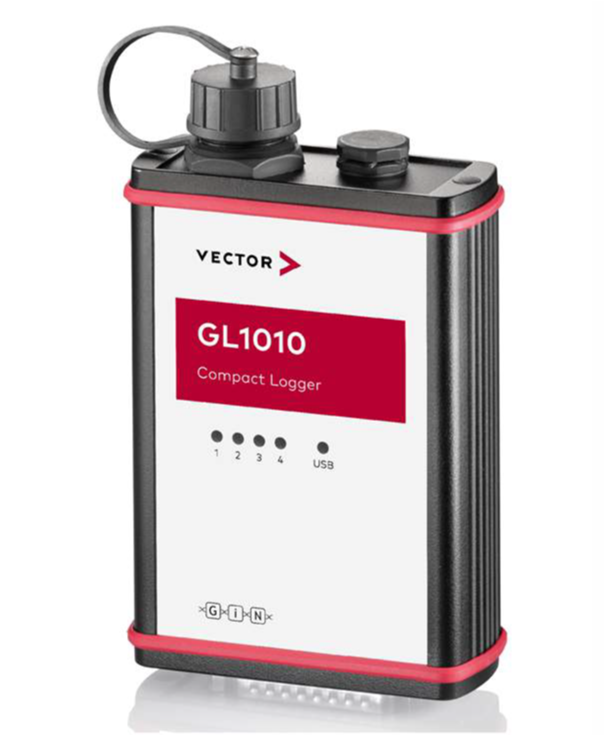
\includegraphics[width=0.7\textwidth]{pics/Vector Logger GL1010.png}
    \caption{Verbauter Vector Logger GL1010 mit CAN-Bus-Anbindung und Speichermedium.}
    \label{fig:datenlogger}
\end{figure}

Zur Auswertung der umfangreichen Datensätze wird ein eigens entwickeltes MATLAB-Skript eingesetzt. Dieses ermöglicht es, die Rohdaten zu filtern, physikalische Einheiten zuzuordnen und thermische Zusammenhänge -- wie etwa die Trägheit des Kühlmittels im Verhältnis zu Lastspitzen der Motoren -- zu visualisieren. Erst durch diese automatisierte Aufbereitung lassen sich die im Wettbewerb oder auf dem Prüfstand gewonnenen Daten für die Validierung der Kühlungsauslegung nutzen.

\subsection{Signalaufbereitung mittels Messbrücken}
\label{subsec:messbruecken}

Da viele physikalische Sensoren -- insbesondere piezoresistive Druckaufnehmer -- auf minimalen Widerstandsänderungen basieren, ist eine direkte Auswertung durch die Analogeingänge der VCU aufgrund des geringen Signal-Rausch-Verhältnisses nicht zielführend. Zur Wandlung dieser Differenzen in ein nutzbares Spannungssignal wird die Wheatstone-Brückenschaltung eingesetzt.

\begin{figure}[htbp]
    \centering
    % \includegraphics[width=0.55\textwidth]{pics/wheatstone_bridge.png}
    \caption{Schaltplan einer Wheatstone-Brückenschaltung zur Wandlung von Widerstandsänderungen in eine proportionale Messspannung $\Delta U$.}
    \label{fig:wheatstone_bridge}
\end{figure}

Ein wesentlicher Vorteil dieses differenziellen Messprinzips ist die Kompensation von Störeinflüssen:
\begin{itemize}
    \item \textbf{Temperaturkompensation:} Da sich Leitungswiderstände bei Erwärmung in allen Brückenzweigen ähnlich ändern, heben sich diese Fehler gegenseitig auf.
    \item \textbf{Nullpunktstabilität:} Die Brücke erlaubt eine hohe Auflösung um den Arbeitspunkt, was besonders bei der Detektion feiner Druckunterschiede im Kühlkreislauf essenziell ist.
\end{itemize}

Die Anzahl der verfügbaren Messbrücken ist durch den Bauraum und die Komplexität der Signalverstärkung begrenzt, weshalb eine gezielte Priorisierung der thermisch kritischsten Messstellen erforderlich ist.

\section{Sensorik der Antriebseinheiten}
\label{sec:antriebssensorik}

\paragraph{Temperaturüberwachung der Antriebsmotoren}
\label{sec:motor}

Jeder Antriebsmotor verfügt über einen in die Statorwicklung eingebetteten PT1000-Widerstandsthermometer. Dieser misst die Wicklungstemperatur direkt an der thermisch kritischsten Stelle des Motors. Das physikalische Messprinzip wird in Abschnitt~\ref{subsec:pt1000} detailliert beschrieben, da es identisch mit den zusätzlich verbauten Kühlmitteltemperatursensoren ist.

\begin{figure}[htbp]
    \centering
    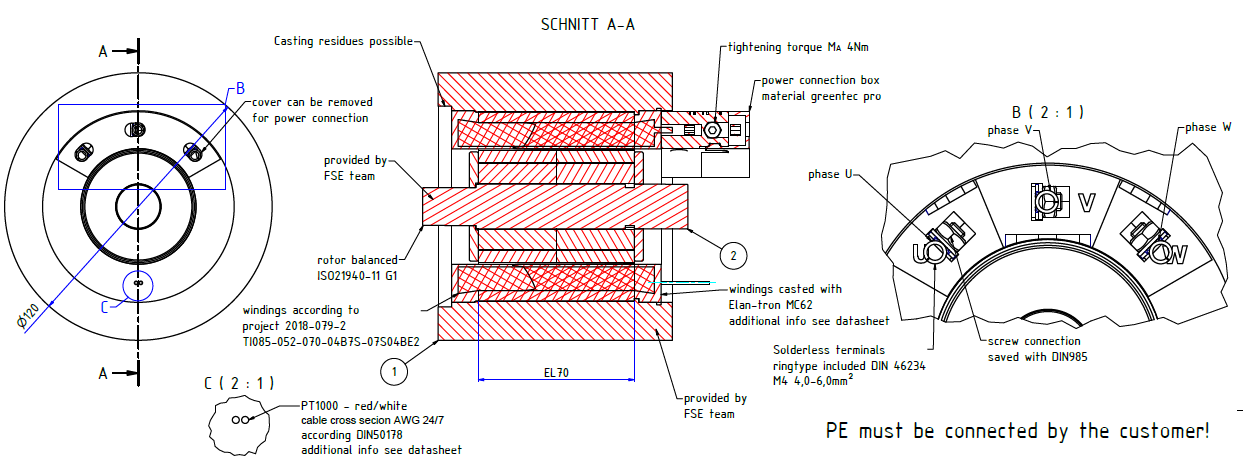
\includegraphics[width=0.7\textwidth]{pics/Motor_Data_sheet.PNG}
    \caption{Einbaulage des PT1000-Sensors in der Statorwicklung eines Antriebsmotors.}
    \label{fig:motor_pt1000}
\end{figure}

\paragraph{Integrierte Sensorik der Inverter}

Jeder Inverter verfügt über einen im IGBT-Modul (Insulated Gate Bipolar Transistor) integrierten Temperatursensor. Dieser erlaubt die direkte Abfrage der Sperrschichttemperatur der Leistungshalbleiter, welche als kritische Betriebsgröße kontinuierlich mitgeloggt wird. Da der Inverterhersteller die Veröffentlichung von Produktabbildungen nicht gestattet, zeigt Abbildung~\ref{fig:inverter_igbt} exemplarisch einen Inverter eines Wettbewerbers, der ein vergleichbares Kühlungskonzept realisiert.

\begin{figure}[htbp]
    \centering
    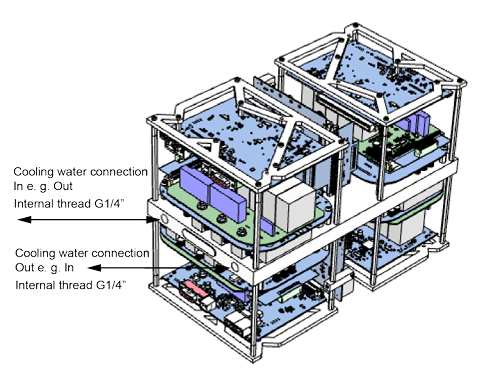
\includegraphics[width=0.7\textwidth]{pics/AMK_Inverter.PNG}
    \caption{Exemplarische Darstellung eines IGBT-Invertermoduls mit integriertem Temperatursensor (Fremdprodukt, da Herstellerfreigabe nicht vorliegt). Das Kühlungskonzept ist vergleichbar mit dem eingesetzten System.}
    \label{fig:inverter_igbt}
\end{figure}

\paragraph{Kühlmittelpumpen und PWM-Ansteuerung}

Im Fahrzeug sind zwei Kühlmittelpumpen verbaut, die die beiden Kühlkreisläufe -- Motorkreislauf und Inverterkreislauf -- unabhängig voneinander versorgen. Die Pumpen ermöglichen keine direkte Messung des Volumenstroms, und eine separate Stromerfassung je Pumpe ist im aktuellen Systemaufbau nicht vorgesehen. Dennoch wird das PWM-Ansteuersignal, das die VCU an die Pumpen sendet, mitgeloggt. Dies erlaubt eine qualitative Nachvollziehbarkeit des Pumpenbetriebszustands in der Datenanalyse. Die fehlende Volumenstromerfassung stellt jedoch eine wesentliche Messlücke dar, die im Rahmen dieser Arbeit durch einen zusätzlichen Durchflusssensor geschlossen wird (siehe Abschnitt~\ref{subsec:volumenstrom}).

\begin{figure}[htbp]
    \centering
    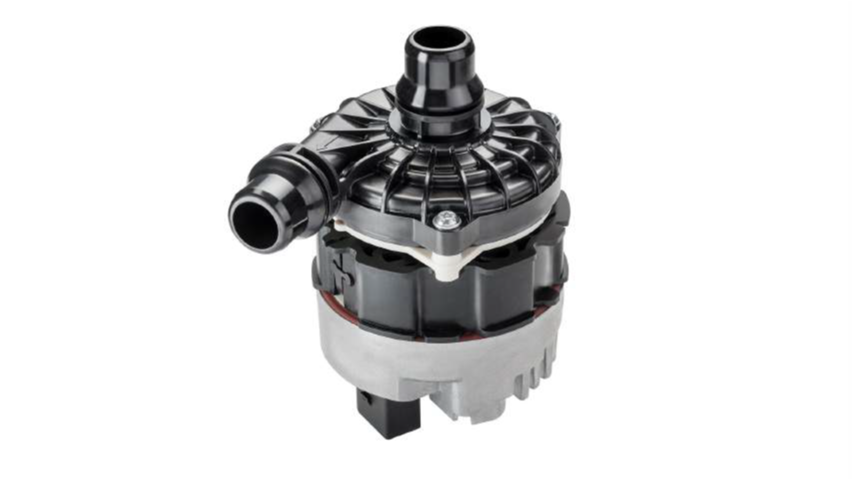
\includegraphics[width=0.7\textwidth]{pics/Pumpe_Vitesco.png}
    \caption{Verbaute Pumpe der Firma Vitesco mit 24V und (60W) Leistung.}
    \label{fig:pumpen_einbau}
\end{figure}

\section{Projektspezifische Erweiterung der Messtechnik}
\label{sec:erweiterung}

Die in Abschnitt~\ref{sec:bestandssensorik} beschriebene Bestandssensorik liefert zwar eine solide Ausgangsbasis, lässt jedoch für eine vollständige thermische Bilanzierung des Kühlsystems wesentliche Messgrößen offen. Im Rahmen dieser Arbeit wird die Messtechnik daher gezielt um zwei Sensortypen erweitert: einen Volumenstromsensor sowie zusätzliche Temperaturmessstellen

\subsection{Volumenstrom-Sensor}
\label{subsec:volumenstrom}

Zur präzisen Bestimmung des Volumenstroms -- und damit zur Berechnung des Massenstroms, der für die thermische Leistungsbilanz des Kühlkreislaufs essenziell ist -- wird ein Turbinen-Durchflusssensor eingesetzt. Abbildung~\ref{fig:durchfluss_sensor_foto} zeigt den verbauten Sensor, Abbildung~\ref{fig:durchfluss_sensor_prinzip} erläutert das zugrunde liegende Wirkprinzip.

\begin{figure}[htbp]
    \centering
    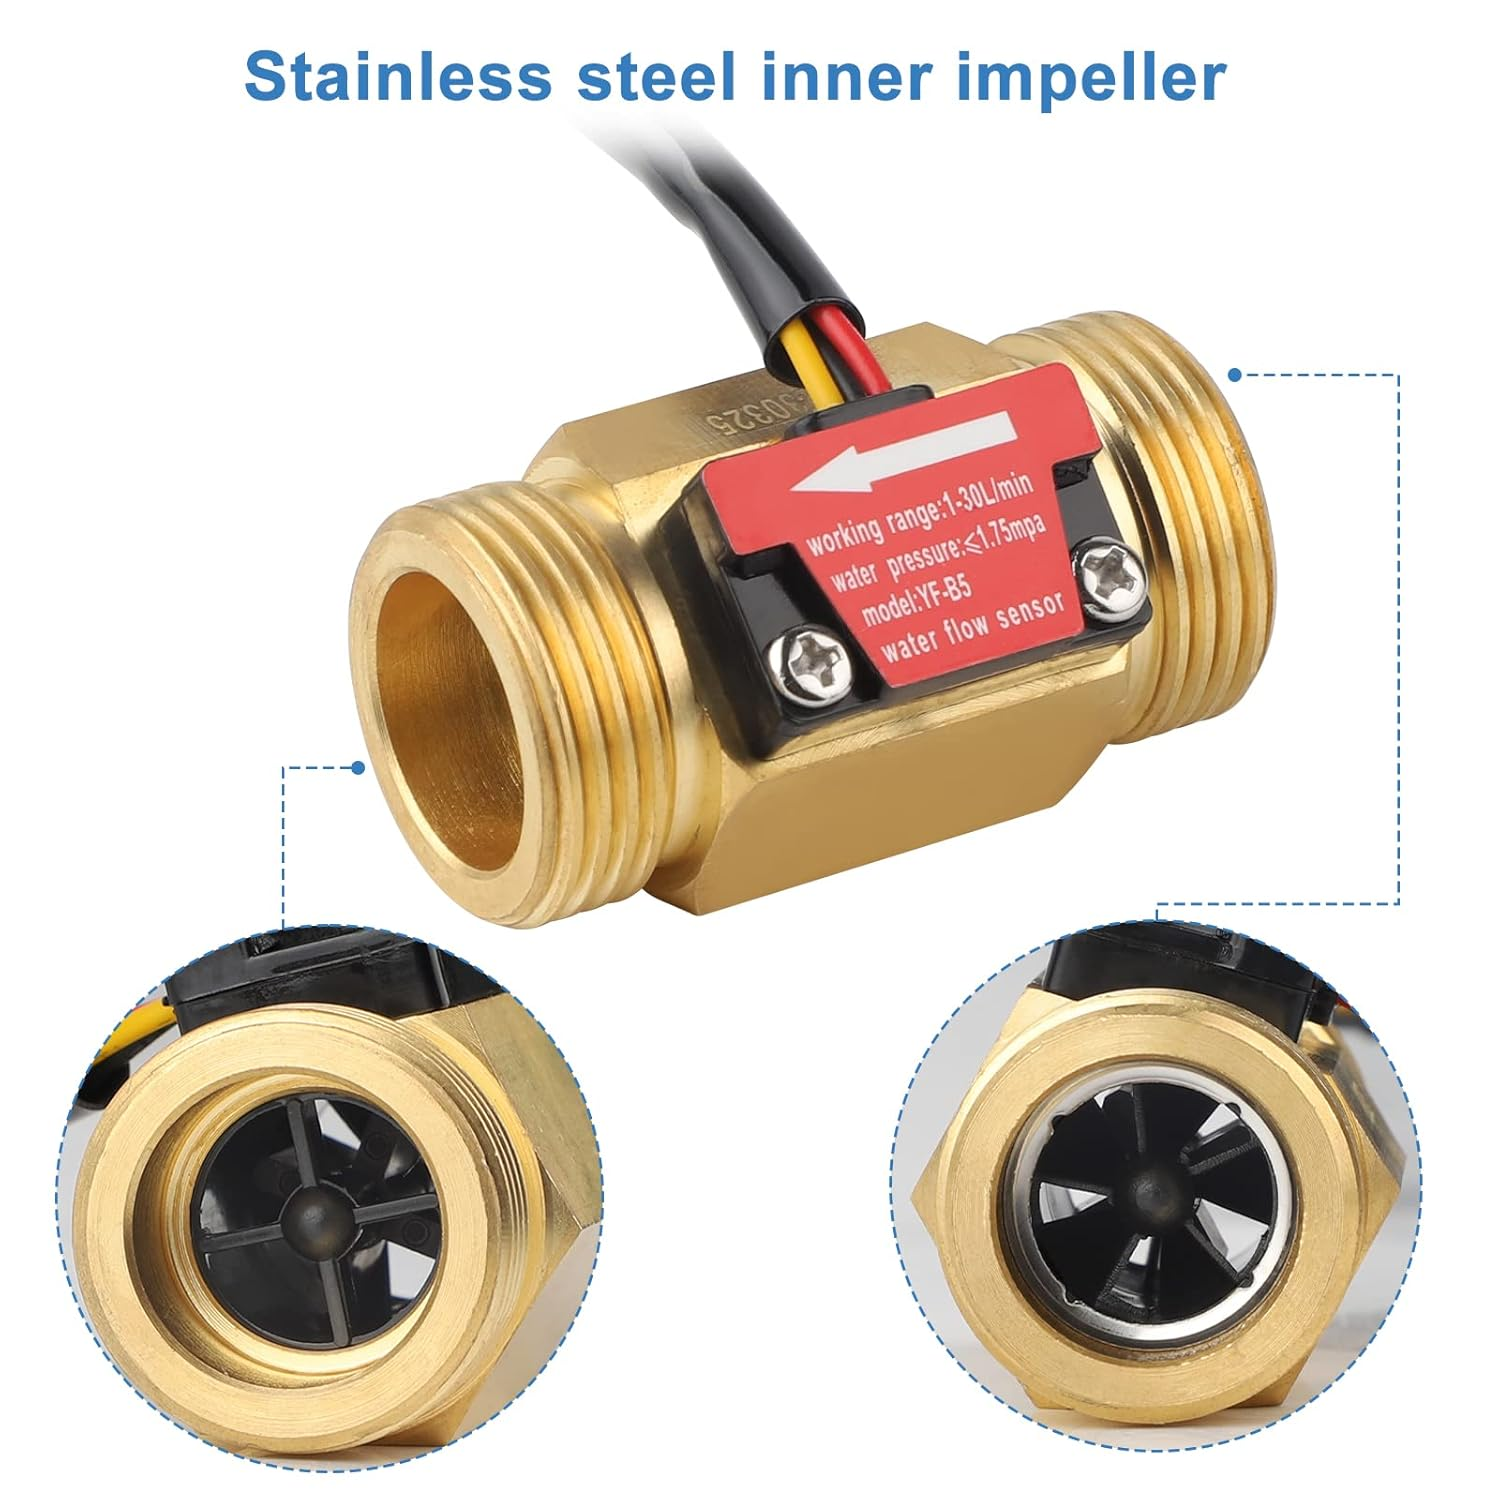
\includegraphics[width=0.6\textwidth]{pics/Volumenstrom_Sensor_neu.jpg}
    \caption{Verbauter Turbinen-Durchflusssensor im Kühlkreislauf des Fahrzeugs.}
    \label{fig:durchfluss_sensor_foto}
\end{figure}

Das Funktionsprinzip basiert auf der Wandlung der Strömungsenergie in eine Rotationsbewegung. Die einströmende Kühlflüssigkeit wird durch Leitschaufeln stabilisiert und auf den Rotor geleitet, dessen Winkelgeschwindigkeit über einen weiten Messbereich linear proportional zur mittleren Strömungsgeschwindigkeit ist. Ein im Rotor integrierter Permanentmagnet erzeugt bei jeder Umdrehung einen Impuls im außenliegenden Hall-Sensor, der als Frequenzsignal an den Datenlogger übertragen wird. Über die bekannte K-Faktor-Konstante des Sensors lässt sich in der Nachauswertung der Volumenstrom in Litern pro Minute berechnen. Da das Messprinzip rein magnetisch und damit berührungslos arbeitet, ist eine hermetische Trennung zwischen Kühlmedium und Sensorelektronik gewährleistet.

\begin{figure}[htbp]
    \centering
    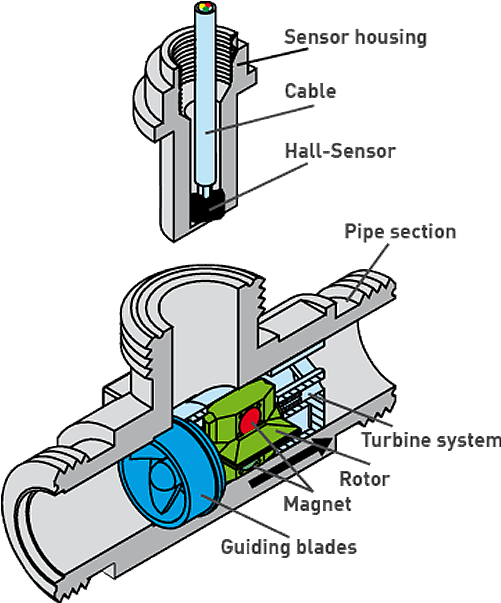
\includegraphics[width=0.7\textwidth]{pics/Turbinen_Durchfluss_Sensor.png}
    \caption{Schnittdarstellung des Turbinen-Durchflusssensors: Die einströmende Flüssigkeit versetzt den Rotor in Rotation, deren Frequenz vom Hall-Sensor erfasst und proportional zum Volumenstrom ausgewertet wird.}
    \label{fig:durchfluss_sensor_prinzip}
\end{figure}

\subsection{Temperatursensorik (PT1000)}
\label{subsec:pt1000}

Zur Erfassung der Kühlmitteltemperatur an kritischen Stellen des Kreislaufs -- insbesondere im Vor- und Rücklauf der Radiatoren -- werden zusätzliche PT1000-Widerstandsthermometer eingesetzt.

\begin{figure}[htbp]
    \centering
    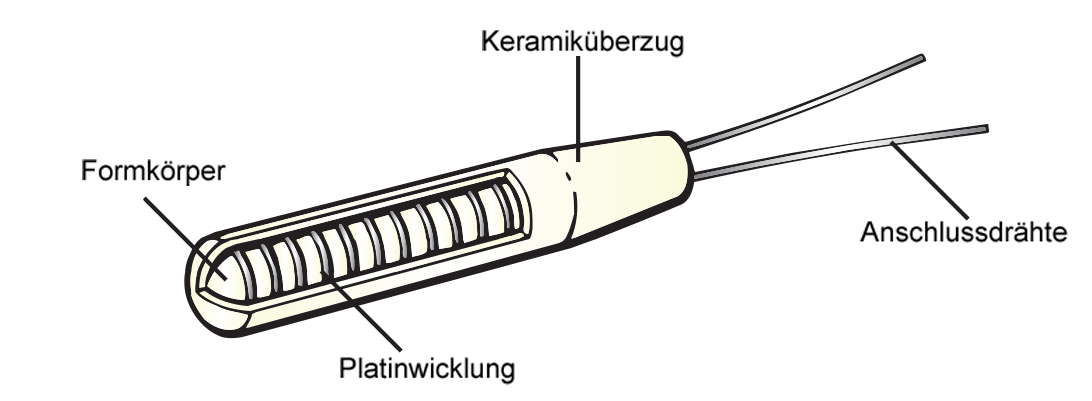
\includegraphics[width=0.6\textwidth]{pics/PT_100_Skizze.png}
    \caption{Schematischer Aufbau eines PT100-Widerstandsthermometers mit Platinwicklung und Keramikschutzmantel.}
    \label{fig:pt1000_aufbau}
\end{figure}

Das Messprinzip basiert auf dem positiven Temperaturkoeffizienten (PTC) von Platin: Mit steigender Temperatur erhöht sich der elektrische Widerstand der Platinwicklung nahezu linear. Ein PT1000 besitzt bei $0\,^\circ\text{C}$ einen Nennwiderstand von $1000\,\Omega$. Die Widerstandsänderung wird über eine Wheatstone-Messbrücke in der VCU ausgewertet und in einen kalibrierten Temperaturwert umgerechnet. Platin zeichnet sich dabei durch eine exzellente Langzeitstabilität aus, was wiederholte Messungen unter Wettbewerbsbedingungen zuverlässig reproduzierbar macht.

\subsection{Differenzdrucksensor (Piezoresistiv)}
\label{subsec:drucksensor}

Zur Bestimmung von Druckverlusten innerhalb des Kühlkreislaufs -- beispielsweise über dem Radiator -- werden piezoresistive Differenzdrucksensoren eingesetzt. Im Gegensatz zu Absolutdrucksensoren verfügen diese über zwei Druckanschlüsse ($P_1$ und $P_2$), sodass direkt die Druckdifferenz $\Delta p = P_1 - P_2$ gemessen wird.

\begin{figure}[htbp]
    \centering
    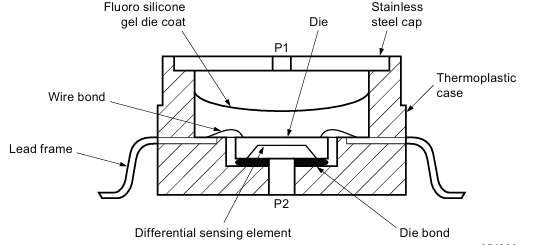
\includegraphics[width=0.7\textwidth]{pics/Piezo_Kristall_MTP.PNG}
    \caption{Interner Aufbau eines piezoresistiven Differenzdrucksensors: Die Druckdifferenz verformt eine Siliziummembran, deren Widerstandsänderung über eine Wheatstone-Brücke ausgewertet wird.}
    \label{fig:drucksensor_aufbau}
\end{figure}

Das Herzstück des Sensors bildet eine dünne Siliziummembran. Eine anliegende Druckdifferenz führt zu deren mechanischer Verformung, wodurch sich der elektrische Widerstand der aufgebrachten piezoresistiven Elemente ändert. Diese sind in einer Wheatstone-Messbrücke verschaltet, die die Dehnung in eine proportionale Ausgangsspannung umwandelt. Zum Schutz der empfindlichen Halbleiterstruktur vor dem Kühlmedium ist das Sensorelement mit einem chemisch inerten Silikon-Gel vergossen, das den hydraulischen Druck verlustfrei überträgt und die Elektronik gleichzeitig isoliert.

% -------------------------------------------------------
\section{Positionierung und Validierung der Sensorik}
\label{sec:validierung}

\subsection{Sensorik und Validierung}
\label{subsec:sensorik}

\subsubsection{Volumenstromsensor}

Der Volumenstromsensor dient dazu, im Stand bzw. im geschlossenen
Kühlkreislauf den Volumenstrom zu bestimmen. Anhand der bekannten
Pumpenkennlinie und der Stromaufnahme der Pumpe kann anschließend geprüft
werden, ob dieser Volumenstrom auch in anderen Betriebssituationen erreicht
wird. Treten Abweichungen auf, lassen sich deren Ursachen und Randbedingungen
eingrenzen.

\subsubsection{Temperatursensorik und Ausbaustrategie}

Die Temperatursensorik wurde im Verlauf der Arbeit entwickelt. Aufgrund der
geringen Verfügbarkeit der WPMD-Platinen konnte bisher nur ein Radpaket
ausgestattet werden. Ein Nachrüsten weiterer Sensoren ist vorgesehen.
Die erarbeitete Strategie gliedert sich in drei Stufen:

\begin{description}
    \item[Stufe 1] Vermessung eines Motors an einem Radpaket. Damit lässt sich
          die grundsätzliche Kühlmitteltemperatur validieren. Aus bekanntem
          Volumenstrom und Temperaturanstieg kann zudem ein Wärmestrom
          bestimmt werden. Wegen der thermischen Trägheit des Motors ist
          dies jedoch nur für quasistatische Fahrsituationen aussagekräftig.
    \item[Stufe 2] Ein Radpaketpaar, ein Inverterpaar und ein Radiatorpaar.
          Damit können alle Komponenten eines Kühlkreislaufs klassifiziert
          werden. Die ermittelten Kennwerte sind Grundlage für die in
          Abschnitt~\ref{TODO_Abschnitt} entwickelten Systemmodelle.
    \item[Stufe 3] Vollständige Vermessung. Alle vier Motoren erhalten ein
          Temperatursensorpaar, ebenso die Inverterkühlung sowie beide
          Radiatoren. Zusätzliche Sensoren erfassen die Lufttemperatur.
\end{description}

\subsubsection{Validierung der Sensorik}

\paragraph{Volumenstrom.} Der Sensor wurde durch Auffangen des Förderstroms
in einem Behälter überprüft. In $t = 60\,\mathrm{s}$ wurden
$V = 21\,\mathrm{l}$ gefördert. Daraus ergibt sich der Referenzvolumenstrom
\begin{equation}
    \dot{V}_\mathrm{ref} = \frac{V}{t}
    = \frac{21\,\mathrm{l}}{60\,\mathrm{s}}
    = 21\,\mathrm{l/min} = 0{,}35\,\mathrm{l/s}.
\end{equation}
Der Sensor zeigte $\dot{V}_\mathrm{Sensor} = 21{,}7\,\mathrm{l/min}$. Die
relative Abweichung beträgt
\begin{equation}
    e = \frac{\dot{V}_\mathrm{Sensor} - \dot{V}_\mathrm{ref}}{\dot{V}_\mathrm{ref}}
    = 3{,}33\,\%.
\end{equation}
Sie liegt innerhalb der Herstellertoleranz von $10\,\%$. Zusätzlich
wurde während des Versuchs eine Pumpenstromaufnahme von $3\,\mathrm{A}$
gemessen, die als Referenz für den weiteren Betrieb dient. Die Unsicherheit
der Referenzmessung aus Zeitnahme und Volumenablesung beträgt $2{,}5\,\%$.

\paragraph{Temperatur: Versuchsdurchführung.} Alle PT100-Sensoren wurden
gleichzeitig in siedendes Wasser getaucht. Nach Einstellen eines stationären
Plateaus wurde über $t = 150\,\mathrm{s}$ per Handnotiz aufgezeichnet. Die Referenztemperatur folgt aus dem
Luftdruck am Messtag ($p = 964\,\mathrm{hPa}$) zu
$T_\mathrm{ref} = 98{,}61\,^\circ\mathrm{C}$.

\paragraph{Temperatur: Auswertung.} Je Sensor $i$ wird der Mittelwert
$\bar{T}_i$ im Plateau gebildet. Die Abweichung zur Referenz ist
$\Delta T_i = \bar{T}_i - T_\mathrm{ref}$. Als Streuung zwischen den
Sensoren dient die Standardabweichung der $\bar{T}_i$.

\begin{table}[htbp]
    \centering
    \caption{Ergebnis des Siedetests der PT100-Sensoren}
    \label{tab:pt100_siedetest}
    \begin{tabular}{lrrr}
        \hline
        Sensor & $\bar{T}_i$ in $^\circ\mathrm{C}$ & $\Delta T_i$ in $\mathrm{K}$ & $s_i$ in $\mathrm{K}$ \\
        \hline
        Sensor 1 & $98{,}52$ & $-0{,}09$ & $0{,}03$ \\
        Sensor 2 & $98{,}78$ & $0{,}17$  & $0{,}05$ \\
        Sensor 3 & $98{,}47$ & $-0{,}14$ & $0{,}04$ \\
        Sensor 4 & $98{,}66$ & $0{,}05$  & $0{,}04$ \\
        Sensor 5 & $98{,}81$ & $0{,}20$  & $0{,}03$ \\
        \hline
    \end{tabular}
\end{table}

\paragraph{Temperatur: Bewertung.} Die maximale Abweichung beträgt
$0{,}20\,\mathrm{K}$, die Streuung zwischen den Sensoren
$0{,}15\,\mathrm{K}$. Zum Vergleich: Die Toleranz nach DIN EN 60751 beträgt
bei $100\,^\circ\mathrm{C}$ für Klasse~A $0{,}35\,\mathrm{K}$ und für
Klasse~B $0{,}8\,\mathrm{K}$. Der Test erfolgte als Einpunktprüfung bei etwa
$100\,^\circ\mathrm{C}$, eine Aussage über den gesamten Betriebsbereich ist
daraus nicht ableitbar.

\paragraph{Temperatur: Zeitkonstante.} Zur Bestimmung der Zeitkonstante
$\tau$ wird zunächst vor dem Versuch die relevante Schwellentemperatur
berechnet. Dazu werden der Anfangswert $T_0$ (Sensor in Raumluft) und der
Endwert $T_\infty$ (gerührtes siedendes Wasser) herangezogen. Für ein
Verzögerungsglied 1.~Ordnung
\begin{equation}
    T(t) = T_\infty - (T_\infty - T_0)\,e^{-t/\tau}
\end{equation}
ist $\tau$ genau dann verstrichen, wenn der Sensor $63{,}2\,\%$ des
Temperatursprungs durchlaufen hat:
\begin{equation}
    T_\tau = T_0 + 0{,}632\,(T_\infty - T_0)
    = 22{,}4\,^\circ\mathrm{C} + 0{,}632 \cdot 76{,}2\,\mathrm{K}
    = 70{,}6\,^\circ\mathrm{C}.
\end{equation}
Anschließend wird der Sensor aus Raumluft schnell in das gerührte
siedende Wasser getaucht und mit $5\,\mathrm{Hz}$ aufgezeichnet. Die
Zeitkonstante $\tau$ ist die Zeit zwischen dem Eintauchen (Signal verlässt
$T_0$) und dem erstmaligen Erreichen von $T_\tau$. Bei $5\,\mathrm{Hz}$
beträgt die Zeitauflösung $0{,}2\,\mathrm{s}$.

\begin{table}[htbp]
    \centering
    \caption{Zeitkonstanten der PT100-Sensoren im gerührten Wasserbad}
    \label{tab:pt100_tau}
    \begin{tabular}{lrrr}
        \hline
        Sensor & $t_{63}$ in $\mathrm{s}$ & $\tau_\mathrm{Fit}$ in $\mathrm{s}$ & $t_{90}$ in $\mathrm{s}$ \\
        \hline
        Sensor 1 & $3{,}4$ & $3{,}3$ & $7{,}6$ \\
        Sensor 2 & $3{,}6$ & $3{,}6$ & $8{,}3$ \\
        Sensor 3 & $3{,}0$ & $2{,}9$ & $6{,}7$ \\
        Sensor 4 & $3{,}1$ & $3{,}1$ & $7{,}1$ \\
        Sensor 5 & $4{,}2$ & $4{,}1$ & $9{,}4$ \\
        \hline
    \end{tabular}
\end{table}

\paragraph{Temperatur: Bewertung der Zeitkonstante.} Die Zeitkonstanten
liegen zwischen $2{,}9\,\mathrm{s}$ und $4{,}1\,\mathrm{s}$. Bei einer
Temperaturrampe $\mathrm{d}T/\mathrm{d}t$ zeigt der Sensor einen
Schleppfehler von $\Delta T = \tau \cdot \mathrm{d}T/\mathrm{d}t$, bei
$0{,}5\,\mathrm{K/s}$ und $\tau = 3{,}6\,\mathrm{s}$ also
$1{,}8\,\mathrm{K}$. Die Werte gelten für die Umströmung im Wasserbad
und können im Kühlkreis mit anderer Strömungsgeschwindigkeit abweichen.

\section{Ausarbeitung eines Testplanes}
\label{sec:Testplanung}

% TODO: Abschnitt nach Abschluss der Messungen ausformulieren.
% Geplante Messprogramme:
%
% Motoren:
%   - Thermische Masse (Gewichtsmessung + Datenblattwerte)
%   - Wärmeübergangskoeffizient (Abkühlversuch mit temperiertem Wasser)
%
% Inverter:
%   - Thermische Masse (Gewichtsmessung + Datenblattwerte)
%   - Wärmeübergangskoeffizient
%
% Pumpen:
%   - Volumenstrom-Kennlinie in Abhängigkeit des PWM-Signals (Testaufbau)
%
% Radiatoren:
%   - Wärmeübertragungskoeffizient (temperiertes Wasser, Vor-/Rücklauftemperatur,
%     Volumenstrom; ggf. Windkanal OTH)
%
% Lüfter:
%   - Luftvolumenstrom im Stand (Lüfter aktiv)
%   - Luftvolumenstrom unter der Fahrt
%   - Wärmeübergangskoeffizient unter Fahrtwind
\chapter{Systemmodelle}
\label{ch:messtechnik}

Zur Zukünfitigen Auslegung und Validierung wurde darauf gesetzt ein Simulink modell von der Fahrzeug kühlung aufzubauen. Diese soll alle Thermischen Komponente beinhalten und soll in Zukunft zur Auslegung und Validierung der Kühlung verwendet werden könnne. Dabei ist besonders relevant alle für die Jühlung relevanten komponente darzustellen oder zumindest die Thermischen einflussgrößen

Um eine Sinnvolle Auslegung zu ermögliche soll die Fahrtsitationen durch eine Vielzahl an Szenarion möglich sein. Dabei sollen sowohl Standard Fahrtsitutionen Analysierbar sein Dazu zählt: Gerade Auswafhrt, Braketest, Acceleartion und Skidpad als auch Dynmaische woei Freie Fahren. Hierzu zählen dann die Disziplinen Autocross Skidpad sowie selbst aufgestllte Testtracks am lokalen Testplatzt. 

Das setzt voraus das Daten aus einer Vielzahl von Quellen eingespielt werden könnnen müssen. Die hauptquellen die hier identifiziert wurden sind Loggingdaten des Fahrzeugs welche Sensor werte im .mf4 format aufweise, diese sind auch möglicherweise verrauscht oder unterliegen anderen Störgrößen der Messtechnik oder die verwendung von Simulationsdaten aus der Rundenzeit Simulation die dem Dynamics bereits vorliegt.

Eine wichtige anmerkung ist an der Stelle das die Thermischen werte direkt das Fahrverhalten des Fahrzeugs beeinflussen. Hier liegen effekte wie das D-Rating also das reduzieren der Leistung aufgrund der Übertemperatur oder auch eine anpassung des Fahrstils des Fahrers um ein Überhitzen der Motoren oder anderer Komponenten zu beeinflussen. Dies betrifft vor allem die Echten Sensor daten kann aber auch bereits in der Laptime simulation über das dort parralel mitentwicklete kühlungsmodell berücksichtigt werden. Dadruch können auslegungen ebenfalls als Ausreichend bewertet werden obwohl die lasten vom Fahrer reduziert wurden und dieser sie auf einem Konstanten Level halten was einer ausreichendne Auslegung täuschend ähnlich sehen würde. 

Der Aufbau des modells gliedert sich in die folgenden Teilmodule:

\chapter{Systemmodelle}
\label{ch:systemmodelle}

\section{Zielsetzung des Kühlungsmodells}
\label{sec:modell_ziel}

Zur zukünftigen Auslegung und Validierung der Fahrzeugkühlung wird ein
Simulink-Modell des Gesamtsystems aufgebaut. Das Modell bildet alle für die
Kühlung relevanten Komponenten ab bzw. berücksichtigt zumindest deren
thermische Einflussgrößen. Es soll im weiteren Projektverlauf sowohl zur
Dimensionierung neuer Kühlkonzepte als auch zur Validierung bestehender
Konzepte eingesetzt werden.

% FIGURE-VORSCHLAG 1: Übersichts-Blockschaltbild des Gesamtmodells
% (Datenquellen -> Datenaufbereitung -> Thermonetzwerk -> Ausgaben/Bewertung).
% Passt hier ans Ende der Section, als Orientierung für das ganze Kapitel.
\begin{figure}[htbp]
    \centering
    % \includegraphics[width=\textwidth]{bilder/modell_uebersicht}
    \caption{Übersicht über die Struktur des Kühlungsmodells}
    \label{fig:modell_uebersicht}
\end{figure}

\section{Betrachtete Fahrszenarien}
\label{sec:fahrszenarien}

Für eine belastbare Auslegung muss die Kühlung unter einer Vielzahl
unterschiedlicher Fahrsituationen analysierbar sein. Das Modell unterscheidet
dabei zwei Gruppen von Szenarien:

\begin{itemize}
    \item \textbf{Standardszenarien:} Geradeausfahrt (Auslauf), Bremstest,
          Acceleration und Skidpad. Diese sind klar definiert und gut
          reproduzierbar.
    \item \textbf{Dynamische Szenarien (freie Fahrt):} Hierzu zählen die
          Disziplinen Autocross sowie selbst aufgestellte Teststrecken auf
          dem lokalen Testgelände.
\end{itemize}

\section{Datenquellen}
\label{sec:datenquellen}

Aus den Szenarien folgt, dass das Modell Daten aus unterschiedlichen Quellen
verarbeiten können muss. Es wurden zwei Hauptquellen identifiziert:

\begin{enumerate}
    \item \textbf{Fahrzeug-Logdaten:} Die Sensorwerte liegen im
          \texttt{.mf4}-Format vor. Sie sind messtechnisch bedingt
          möglicherweise verrauscht oder durch weitere Störgrößen der
          Messtechnik beeinflusst und müssen daher aufbereitet werden
          (vgl.~Kapitel~\ref{ch:messtechnik}).
    \item \textbf{Simulationsdaten:} Die im Team Dynamics bereits vorhandene
          Rundenzeitsimulation liefert simulierte Fahrzustände als Eingang.
\end{enumerate}

% FIGURE-VORSCHLAG 2: Beispielsignal aus einer .mf4-Messung, Rohdaten vs.
% aufbereitet (z.B. Temperatur oder Strom). Zeigt anschaulich, warum die
% Datenaufbereitung nötig ist.
\begin{figure}[htbp]
    \centering
    % \includegraphics[width=0.8\textwidth]{bilder/rohdaten_vs_gefiltert}
    \caption{Beispiel eines Messsignals im Rohzustand und nach der Aufbereitung}
    \label{fig:rohdaten_gefiltert}
\end{figure}

\section{Rückwirkung der Thermik auf das Fahrverhalten}
\label{sec:rueckwirkung}

Die thermischen Zustände beeinflussen unmittelbar das Fahrverhalten des
Fahrzeugs. Zum einen reduziert das Derating die Leistung bei Übertemperatur.
Zum anderen passt der Fahrer seinen Fahrstil an, um ein Überhitzen der Motoren
oder anderer Komponenten zu vermeiden.

Dieser Effekt betrifft vor allem die realen Messdaten. Er kann aber auch in
der Rundenzeitsimulation berücksichtigt werden, in der parallel ein
Kühlungsmodell mitentwickelt wird.

Hieraus ergibt sich eine wichtige Einschränkung bei der Bewertung: Reduziert
der Fahrer die Last oder hält er sie auf einem konstanten Niveau, kann eine
Auslegung fälschlicherweise als ausreichend bewertet werden, obwohl sie bei
voller Leistungsabgabe nicht genügen würde. Die Messdaten sind daher stets im
Zusammenhang mit dem tatsächlichen Fahrerverhalten und möglichen
Deratingeingriffen zu interpretieren.

% FIGURE-VORSCHLAG 3: Wirkkette/Regelkreis Temperatur -> Derating bzw.
% Fahrerreaktion -> Last -> Verlustleistung -> Temperatur.
% Alternativ oder zusätzlich: Messung mit Leistung und Temperatur über der Zeit,
% in der die Leistungsreduktion bei Übertemperatur sichtbar ist.
\begin{figure}[htbp]
    \centering
    % \includegraphics[width=0.8\textwidth]{bilder/rueckwirkung_thermik}
    \caption{Rückwirkung der Bauteiltemperatur auf die abrufbare Leistung}
    \label{fig:rueckwirkung}
\end{figure}

\section{Modellaufbau}
\label{sec:modellaufbau}

Der Aufbau des Modells gliedert sich in die folgenden Teilmodule:

% TODO: Liste der Teilmodule einfügen
\begin{itemize}
    \item Akkumulator
    \item Bremse
    \item Motoren
    \item Inverter
\end{itemize}

% FIGURE-VORSCHLAG 4: Simulink-Screenshot der obersten Modellebene
% mit den Teilmodulen.

\subsection{Akkumodell}
\label{subsec:akkumodell}

Das Modell für die Verlustleistung des Akkus wurde bewusst einfach gehalten.
Bei Pouchzellen treten die typischen Hotspots an den Zelltabs auf, insbesondere
am negativen Zelltab~\cite{TODO_Quelle}. Der Zellkörper erwärmt sich ebenfalls,
jedoch deutlich schwächer als die dünnen Tabs. Entsprechend beschränkte sich die
Kühlung des Akkus bisher auf den negativen Zelltab.

% FIGURE-VORSCHLAG 5: Skizze oder Foto einer Pouchzelle mit markierten Zelltabs
% (positiv/negativ) und Hotspot-Bereich, ggf. mit qualitativer Temperaturverteilung.
\begin{figure}[htbp]
    \centering
    % \includegraphics[width=0.7\textwidth]{bilder/pouchzelle_hotspots}
    \caption{Pouchzelle mit Zelltabs und typischem Hotspot am negativen Tab}
    \label{fig:pouchzelle_hotspots}
\end{figure}

Für die Modellierung wurde der Battery Builder aus Simscape Battery in MATLAB
verwendet. Damit lassen sich einzelne Zellen, Stacks und der gesamte Akkuaufbau
abbilden und neben den elektrischen Akkueffekten auch thermisch modellieren.
Der Ansatz erlaubt es, Logging- und Rundenzeitsimulationsdaten als Eingang zu
nutzen, um die Leistungsdaten des Akkus vorzugeben.

Neben den thermischen Simulationen kann das Modell auch zur Akkuauslegung
eingesetzt werden. Diese ist nicht Gegenstand der vorliegenden Arbeit, bietet
aber eine gute Grundlage für eine einfache zukünftige Auslegung von Akku und
Akkukühlung.

% FIGURE-VORSCHLAG 6: Screenshot des Battery Builders bzw. des Akku-Aufbaus
% (Zelle -> Stack -> Pack) mit der verwendeten Konfiguration.
\begin{figure}[htbp]
    \centering
    % \includegraphics[width=0.8\textwidth]{bilder/battery_builder_aufbau}
    \caption{Aufbau des Akkumodells im Battery Builder}
    \label{fig:battery_builder}
\end{figure}

% FIGURE-VORSCHLAG 7 (optional): Simulierte Tab-Temperatur über der Zeit für ein
% Szenario, z.B. Autocross, mit Eingangsleistung des Akkus darüber.

\subsubsection{Bremsen}
\subsubsection{Motoren}
\subsubsection{Motoren}
\label{subsubsec:motoren}

Für die Modellierung der Motoren sollte, wie in Abschnitt~\ref{TODO_Abschnitt}
beschrieben, ein Wirkungsgradkennfeld über Messungen erstellt werden. Dies war
nicht möglich. Stattdessen wird das vom Hersteller mitgelieferte
Wirkungsgradkennfeld verwendet.

Das Modell besteht aus einer einfachen thermischen Masse. Eingangsgrößen sind
Drehmoment $M$ und Drehzahl $n$. Aus dem Kennfeld wird der Wirkungsgrad
$\eta(M,n)$ bestimmt und daraus die in den Motor eingebrachte Verlustleistung
berechnet:

\begin{equation}
    P_\mathrm{V} = P_\mathrm{mech} \left( \frac{1}{\eta(M,n)} - 1 \right)
                 = 2\pi\, n\, M \left( \frac{1}{\eta(M,n)} - 1 \right)
    \label{eq:verlustleistung_motor}
\end{equation}

Die Wärmeabfuhr über die Wasserkühlung der Motoren wird ebenfalls
berücksichtigt.

% FIGURE-VORSCHLAG 8: Wirkungsgradkennfeld des Herstellers (Drehmoment über
% Drehzahl, Wirkungsgrad als Konturplot), ggf. mit eingezeichneten
% Betriebspunkten aus einer Messfahrt.
\begin{figure}[htbp]
    \centering
    % \includegraphics[width=0.8\textwidth]{bilder/motor_wirkungsgradkennfeld}
    \caption{Wirkungsgradkennfeld des Motors (Herstellerangabe)}
    \label{fig:motor_kennfeld}
\end{figure}

Die Modellparameter, z.\,B.\ Wärmekapazität und Wärmeübergänge, lassen sich
nur aus anderen Versuchen ableiten oder müssen an vielen Stellen geschätzt
werden. Eine ausführliche Parameteridentifikation steht daher noch aus.

Das Modell ist als einfaches Simscape-Modell aufgebaut. Jeder Motor bildet ein
eigenes Subsystem. Dadurch lassen sich unterschiedliche Aufbauten und
Kühllayouts sowie die Pumpenauswahl validieren.

% FIGURE-VORSCHLAG 9: Simscape-Screenshot eines Motor-Subsystems
% (thermische Masse, Verlustleistungsquelle, Kühlkreis-Anbindung)
% oder alternativ ein thermisches Ersatzschaltbild als Skizze.
\begin{figure}[htbp]
    \centering
    % \includegraphics[width=0.8\textwidth]{bilder/motor_subsystem}
    \caption{Motor-Subsystem im Simscape-Modell}
    \label{fig:motor_subsystem}
\end{figure}

\subsubsection{Inverter}
Kein plan mehr. Ich hab den nie sauber modelliert. Die sind arsch komplex


\section{Systemmodellierung in Matlab/Simulink}

\subsection{Aufbau des thermischen Netzwerkmodells (0D/1D)}
In diesem Abschnitt wird die grundlegende Architektur des Simulationsmodells beschrieben. Fokus liegt auf der Abstraktion der physikalischen Komponenten in konzentrierte Parameter.
\begin{itemize}
    \item \textbf{Diskretisierung der Komponenten:} Aufteilung des Kühlkreislaufs in thermische Massen (Knoten) und thermische Widerstände.
    \item \textbf{Energiebilanzgleichungen:} Aufstellung der Differentialgleichungen für die instationäre Temperaturänderung $\dot{Q} = m \cdot c_p \cdot \frac{dT}{dt}$.
    \item \textbf{Fluid-Eigenschaften:} Implementierung von temperaturabhängigen Stoffwerten für Kühlwasser (Glykol-Gemisch) und Luft.
\end{itemize}

\subsection{Modellierung der Wärmeübertrager}
Der Kühler ist das zentrale Element zur Wärmeabfuhr. Hier wird die mathematische Abbildung der Wärmeübertragung definiert.
\begin{itemize}
    \item \textbf{$\varepsilon$-NTU-Verfahren oder LMTD-Methode:} Wahl des Berechnungsansatzes für den Wärmestrom zwischen Fluid und Umgebungsluft.
    \item \textbf{Kühler-Kennfelder:} Implementierung von experimentell ermittelten Wirkungsgraden in Abhängigkeit von Massenstrom und Anströmgeschwindigkeit.
    \item \textbf{Ölkühler-Integration:} Kopplung des Ölkreislaufs mit dem Wasserkreislauf (Wasser-Öl-Wärmetauscher).
\end{itemize}

\subsection{Aktoren und Regelungsorgane}
Dieser Teil beschreibt die hydraulischen und mechanischen Komponenten, die den Volumenstrom beeinflussen.
\begin{itemize}
    \item \textbf{Pumpenkennlinien:} Modellierung der elektrischen Wasserpumpe mittels Look-up-Tables (Druckdifferenz vs. Volumenstrom vs. Spannung).
    \item \textbf{Thermostatregelung:} Abbildung der Kennlinie des Thermostatventils (Öffnungsgrad über der Temperatur) zur Steuerung des Kurzschluss- vs. Hauptkreislaufs.
    \item \textbf{Lüftermodelle:} Modellierung des induzierten Luftmassenstroms durch die Kühlerlüfter bei geringen Fahrgeschwindigkeiten.
\end{itemize}

\subsection{Einspeisung von Streckendaten und Fahrzyklen}
Damit das Modell realistische Ergebnisse liefert, müssen dynamische Randbedingungen definiert werden.
\begin{itemize}
    \item \textbf{Datenvorverarbeitung:} Import von GPS-Daten, Geschwindigkeitsprofilen und Lastzuständen aus realen Testfahrten oder Rundenzeitsimulationen.
    \item \textbf{Lastkollektive:} Definition der thermischen Lastvorgaben für Motor/Inverter/Batterie in Abhängigkeit von der Fahrpedalstellung und Drehzahl.
    \item \textbf{Simulationsumgebung:} Aufbau der Signalstruktur zur dynamischen Ansteuerung des Modells während der Zeitbereichssimulation.
\end{itemize}

\subsection{Parameteridentifikation und Validierung}
Abschluss der Modellbildung durch den Abgleich mit der Realität.
\begin{itemize}
    \item \textbf{Abgleich mit Messdaten:} Nutzung von Sensordaten (Temperaturfühler Ein-/Auslass) zur Kalibrierung von Wärmeübergangskoeffizienten.
    \item \textbf{Optimierungsalgorithmen:} Einsatz der Matlab Optimization Toolbox zur Bestimmung unbekannter Modellparameter (z.B. Reibungsverluste in den Leitungen).
    \item \textbf{Sensitivitätsanalyse:} Untersuchung des Einflusses kritischer Parameter auf die maximale Systemtemperatur.
\end{itemize}


% \subsection{Simulink modell}

% \subsubsection{Driver Modell}
% Bei der Erstellung des Fahrermodells wurde Wert gelegt ein Möglichts Simples Fahrermodell welches druch Entweder Rundenzeitsimulation oder direkte Fahrzeuglogging daten gefüttert wird zu erstellen. In sofern fällt hier nur noch die Rolle der Datenaufbereitung und weitergabe an die Zustandsmodelle. In Zukunftigen arbeiten kann hier wert auf eine Implementierung der VCU Logik gelegt werden um eine direkte einbindung der Kühlungsmodelle in die Rundenzeit Simulation zu ermöglichen und hier On the line Paramteterstudien mit Live effekten auf das Fahrzeugverhalten durchzuführen.
% (Bild von Fahrermodell)


% \subsubsection{Inverterkreislaufmodell}
% In diesem finden sich die 4 Inverter Verschlatne wie diese auch in der Eigentlchen Fahrzeug kühlung zu finden sind. Eine Kühler und Pumpen Logik wurde ebenfalls implementiert.

% \subsubsection{Motorkreislaufmodell}
% In diesem Modell finden sich die 4 Motoren verschalten wie diese auch in der eigentlichen Fahrzeugkühlung zu finden sind. Auch hier wurde eine Kühler und Pumpen Logik implementiert.

% \subsubsection{Invertermodell}
% Die Verlustleistung der INverter konte Bislang nicht experimentel bestimmt werden. Dies findet sich ggf. im Abschnitt messungen am Motorprüftstand wieder.
% Das modell umfasst eine umfassende Analytische Berechnung der Inverter Verlustlsietung ist aber nach wie for auf wichtige Expirementel zu ermittelnde Parameter angewisen.

% \subsubsection{Motormodell}
% Das Motormodell ist ebenfalls auf Experimentell zu bestimmende Parameter angewiesen. Bislang wurde eine vom Hersteller mitgeliefterte Effizeinzkarte eingebaut, welche anhand von Drehzahl und Drehmoment den Wirkungsgrad und damit die Verlustleistung bestimmt.

% \subsubsection{Kühlermodell}
% Hier wurde eine Simpler Radiator implementiert welcher ebenfalls nach Datenblatt werte welche noch expirimentell zu VAlideren ist angewiesen ist. Dieser bestimmt in Anbhängigkeit an die Luftgeschwindigkeit die Kühlleistung

% \subsubsection{Lüftermodell}
% Dieser gibt lediglich die Luftvolumenstrom vor. Je nach Fahrzeuggeschwindigkeit überwiegt die Lüfter leistung oder die Fahrzeugluftgeschwindigkeit. In alter implementierung bremst der Lüfter sogar bei voller Fahrt als Negative Konsequenz den Lüfterstrom.

% \subsection{Visualierung der Simulation und Realitätsabweichung}
% unklar was hier auftauchen wird. -> Diskutieren wenn es soweit ist

\subsection{Struktur des Simulink-Gesamtmodells}

\subsubsection{Eingangsdaten und Fahrermodell}
Das Fahrermodell dient als zentrale Datenschnittstelle. Es bereitet transiente Geschwindigkeitsprofile sowie Lastzustände auf, die entweder aus einer Rundenzeitsimulation (Lapsim) oder aus Real-Data-Loggings der VCU stammen. Die modulare Struktur ermöglicht es, zukünftig Regelungslogiken der VCU (z.B. Derating-Strategien) direkt in den Simulationsschleifen zu evaluieren.

\subsubsection{Thermische Lastmodelle (Inverter und Motor)}
Die Wärmeeinträge in das System werden komponentenweise berechnet:
\begin{itemize}
    \item \textbf{Invertermodell:} Da zum aktuellen Zeitpunkt keine Prüfstandsdaten vorliegen, basiert die Verlustleistungsberechnung auf einem analytischen Ansatz, welcher Schalt- und Durchlassverluste der Leistungselektronik mathematisch beschreibt.
    \item \textbf{Motormodell:} Die thermische Last des Elektroantriebs wird über wirkungsgradbasierte Kennfelder (Efficiency Maps) ermittelt. Hierbei wird die Verlustleistung $\dot{Q}_{loss}$ in Abhängigkeit vom aktuellen Arbeitspunkt (Drehmoment $M$, Drehzahl $n$) berechnet.
\end{itemize}

\subsubsection{Hydraulische Verschaltung und Kreisläufe}
In diesen Submodellen wird die physische Anordnung der Komponenten (Inverter- und Motorkreislauf) abgebildet. 
\begin{itemize}
    \item Implementierung der pumpenspezifischen Kennlinien zur Bestimmung des Volumenstroms.
    \item Berücksichtigung der thermischen Trägheiten der Fluidmassen und Gehäusekomponenten (Wärmekapazitäten).
\end{itemize}

\subsubsection{Wärmeübertrager- und Lüfterinteraktion}
Das Kühlermodell berechnet den Wärmestrom an die Umgebung basierend auf Hersteller-Datenblättern. Ein kritischer Aspekt der Modellierung ist die Kopplung mit dem Lüftermodell:
\begin{itemize}
    \item Berechnung der effektiven Anströmgeschwindigkeit unter Berücksichtigung des Staudrucks bei hohen Fahrgeschwindigkeiten.
    \item Abbildung des parasitären Effekts, bei dem der Lüfterwiderstand den natürlichen Luftstrom bei hoher Fahrzeuggeschwindigkeit (Vmax) theoretisch begrenzen kann.
\end{itemize}

\subsection{Visualisierung der Simulation und Validierung}
% Dieser Abschnitt bleibt vorerst als Platzhalter für den Vergleich 
% zwischen Simulationsergebnissen und Realmessungen (Prüfstand/Track).

\section{CFD \& thermische Simulation}
In diesem Abschnitt soll 


\subsection{Modellierung der luftgekühlten Komponenten}
In diesem Abschnitt werden die Systeme untersucht, die direkt durch den Fahrtwind oder Lüfter beaufschlagt werden.
\begin{itemize}
    \item \textbf{Akku-Luftkühlung:} Analyse der Durchströmung des Battery-Packs. Fokus auf der gleichmäßigen Umströmung der Zellen, um Temperaturgradienten innerhalb der Module zu minimieren.
    \item \textbf{Inverter-Kühlung (Luftseite):} Untersuchung der Kühlkörpergeometrie und der Positionierung im Luftstrom zur Vermeidung von Rezirkulationszonen.
    \item \textbf{Druckverlust-Charakteristik:} Ermittlung des Strömungswiderstands der Gehäuse und Kühlrippen für das übergeordnete Systemmodell.
\end{itemize}

\subsection{Simulation der wassergekühlten Wärmetauscher}
Die wasserseitige Simulation konzentriert sich auf die effiziente Wärmeabfuhr aus den Hochleistungskomponenten.
\begin{itemize}
    \item \textbf{Radiator-Durchströmung:} Detail-CFD des Kühlers zur Bestimmung der lokalen Wärmeübergangskoeffizienten zwischen Wasserkanälen und Lamellen.
    \item \textbf{Kühlmantel-Optimierung:} Simulation der Wasserführung in Motor und Inverter zur Maximierung der turbulenten Durchmischung (Erhöhung der Nusselt-Zahl).
    \item \textbf{Kavitationsprüfung:} Untersuchung kritischer Engstellen im Kreislauf auf potenzielle Kavitationserscheinungen bei hohen Pumpendrehzahlen.
\end{itemize}

\subsection{Gekoppelte CHT-Simulation (Conjugate Heat Transfer)}
Die Kopplung von Fluid- und Festkörpertemperaturfeldern ist entscheidend für die Bauteilsicherheit.
\begin{itemize}
    \item \textbf{Thermische Schnittstellen:} Modellierung des Wärmeübergangs von der Leistungselektronik (IGBTs/MOSFETs) über die Wärmeleitpaste zum Kühlmedium.
    \item \textbf{Hotspot-Analyse:} Identifikation von Bereichen mit unzureichender Kühlleistung unter transienten Spitzenlasten (z.B. Beschleunigungsphasen).
\end{itemize}

\subsection{Validierung gegenüber Messdaten}
\begin{itemize}
    \item \textbf{Sensorabgleich:} Vergleich der simulierten Druckverluste ($\Delta p$) und Temperaturspreizungen ($\Delta T$) mit Daten aus dem Fahrzeug-Logging.
    \item \textbf{Netzstudie:} Nachweis der Ergebnisstabilität durch Variation der Elementgröße in den Grenzschichten (y-plus-Betrachtung).
\end{itemize}
Hier soll auf die Positionierung der Kühlungskomponente so wie deren aktuelle Postion angesprochen werden.


Stand Akkukühlung:
Warum brauchen wir eine Akkukühlung?

Stand Akkukühlung:
Stand der Inverterkühlung

\section{Hydraulische Charakterisierung der Komponenten}
\label{sec:hydraulik}

Um den Druckverlust des Kühlkreislaufs und den benötigten Druckaufbau der Pumpe
bestimmen zu können, müssen zunächst die Druckverluste der einzelnen Bauteile
ermittelt werden.

\subsection{Messaufbau}
\label{subsec:hydraulik_messaufbau}

Die Messungen erfolgten am Fahrzeug RP25e/d. Dieses besitzt zwei getrennte
Kühlkreisläufe: einen für den Inverter und einen für die vier in Reihe
geschalteten Motoren.

% FIGURE-VORSCHLAG 19: Fließbild der beiden Kühlkreisläufe des RP25e/d
% (Inverter-Kreis; Motor-Kreis mit vier Motoren in Reihe, Radiatoren, Pumpen).

\subsection{Vorgehen}
\label{subsec:hydraulik_vorgehen}

Zunächst wurden beide Kreisläufe im Ausgangszustand vermessen. Dazu wurde
der Volumenstrom ermittelt, indem die innerhalb einer Minute geförderte
Wassermenge bestimmt wurde. Anschließend wurde jeweils eine Komponente aus dem
Kreis entfernt und die Messung wiederholt. Aus den unterschiedlichen
Durchflüssen lässt sich der hydraulische Widerstand der entfernten Komponente
bestimmen.

Betrachtet wurden folgende Komponenten: Schlauch mit \SI{10}{mm}
\TODO{Innen- oder Außendurchmesser} je \SI{1}{m} Länge, Motor, Radiator und
Inverter.

\subsection{Berechnung der Widerstandswerte}
\label{subsec:hydraulik_berechnung}

Für den turbulent durchströmten Kreis wird der Druckverlust als quadratisch
vom Volumenstrom abhängig angenommen:
\begin{equation}
    \Delta p = R \, \dot{V}^{2}.
    \label{eq:druckverlust}
\end{equation}
Bei Reihenschaltung addieren sich die Widerstände der Komponenten zu
$R_\mathrm{ges} = \sum_i R_i$. Die Pumpe arbeitet in dem Betriebspunkt, in dem
ihr Druckaufbau $\Delta p_\mathrm{P}(\dot{V})$ dem Druckverlust des Kreises
entspricht. Für den Ausgangszustand (Index 1) und den Zustand ohne Komponente
$K$ (Index 2) gilt damit
\begin{align}
    \Delta p_\mathrm{P}(\dot{V}_1) &= R_\mathrm{ges}\,\dot{V}_1^{2}, \\
    \Delta p_\mathrm{P}(\dot{V}_2) &= \left(R_\mathrm{ges} - R_K\right)\dot{V}_2^{2}.
\end{align}
Daraus folgt für den Widerstand der Komponente
\begin{equation}
    R_K = \frac{\Delta p_\mathrm{P}(\dot{V}_1)}{\dot{V}_1^{2}}
        - \frac{\Delta p_\mathrm{P}(\dot{V}_2)}{\dot{V}_2^{2}}.
    \label{eq:widerstand_komponente}
\end{equation}
Der Druckaufbau der Pumpe wird dabei aus der bekannten Pumpenkennlinie bei
den gemessenen Volumenströmen abgelesen.

\begin{table}[htbp]
    \centering
    \caption{Ermittelte hydraulische Widerstände der Komponenten}
    \label{tab:hydraulik_widerstaende}
    \begin{tabular}{l S[table-format=2.2] l}
        \toprule
        Komponente & {$R$ in \si{...}} & Bemerkung \\
        \midrule
        Schlauch (\SI{10}{mm}, je \SI{1}{m}) & {\TODO{}} & \\
        Motor & {\TODO{}} & \\
        Radiator & {\TODO{}} & \\
        Inverter & {\TODO{}} & \\
        \bottomrule
    \end{tabular}
\end{table}

% FIGURE-VORSCHLAG 20: Pumpenkennlinie mit den gemessenen Betriebspunkten
% (Ausgangszustand und je ein Punkt pro entfernter Komponente) und den
% zugehörigen Anlagenkennlinien.

\subsection{Modellierung und Layoutvergleich}
\label{subsec:hydraulik_modell}

Anschließend wurde der Kühlkreislauf in MATLAB nachgebildet. Die berechneten
Werte wurden mit einem Korrekturfaktor an die Messwerte angeglichen. Der
Korrekturfaktor beträgt \TODO{} und ergibt sich aus \TODO{Definition}.
Danach wurden verschiedene Layouts in MATLAB aufgebaut, deren Durchflüsse
und mögliche Wärmeabfuhr berechnet und verglichen.

% FIGURE-VORSCHLAG 21: Vergleich Messung und Modell (Volumenstrom je Konfiguration).
% FIGURE-VORSCHLAG 22: Balkendiagramm Durchfluss/Wärmeabfuhr je Layout.
\chapter{Konstruktionsbegründung}
\label{chap:konstruktionsbegruendung}

\section{Positionierung von Radiator und Lüfter}
\label{sec:Positionierung}

Für die Anordnung der Radiatoren am Fahrzeug existieren mehrere Möglichkeiten,
die jeweils unterschiedliche Kompromisse erfordern. Die Wahl der Position
beeinflusst die Qualität der Anströmung, die Aerodynamik des Gesamtfahrzeugs,
die Lage des Schwerpunkts sowie den Konstruktions- und Fertigungsaufwand.

\subsection{Randbedingungen}
\label{subsec:randbedingungen_position}

Folgende Randbedingungen waren bei der Positionierung zu berücksichtigen:

\begin{itemize}
    \item \textbf{Anströmung:} Je weiter vorne der Radiator sitzt, desto
          sauberer ist die anströmende Luft. Gleichzeitig verwirbelt er die
          Luft für alle dahinterliegenden Bauteile stärker, insbesondere für
          die Aerodynamik im hinteren Fahrzeugbereich.
    \item \textbf{Einbauhöhe:} Höhere Positionen ermöglichen in der Regel
          eine sauberere Anströmung, tiefere Positionen sind hingegen
          deutlich günstiger für die Schwerpunkthöhe.
    \item \textbf{Fahrersichtfeld und Driver Fluid Protection:} Nach
          Regel T0.0.00 dürfen im Sichtfeld des Fahrers keine
          wasserführenden Schläuche verlaufen. Zusätzlich ist die Driver
          Fluid Protection (T0.0.0) einzuhalten.
    \item \textbf{Trägheit:} Massen, die weit von der Hochachse entfernt
          montiert werden, erhöhen das Trägheitsmoment des Fahrzeugs.
\end{itemize}

\subsection{Betrachtete Positionsvarianten}
\label{subsec:positionsvarianten}

In den letzten Jahren haben sich bei den Teams drei grundsätzliche Positionen
durchgesetzt, die jeweils mehrere Untervarianten aufweisen.

\paragraph{Position im Frontwing.}
Diese Variante wird beispielsweise vom Team Amberg-Weiden Running Snails
eingesetzt~\cite{TODO_Quelle_Running_Snails}. Die Radiatoren sind dabei in
einem neu gestalteten Frontwing untergebracht, und ein Cooling Duct verläuft
durch den Frontwing. Laut Reglement wird dadurch ein sonst ungenutzter
Bauraum verwendet, und der Radiator erhält die beste und sauberste
Anströmung. Nachteilig sind die relativ hohe Schwerpunktlage sowie ein
erhöhtes Trägheitsmoment des Fahrzeugs, da die Masse weit entfernt vom
Drehpunkt montiert wird. Auch die Einhaltung der Driver Fluid Protection
(T0.0.0) ist bei dieser Variante anspruchsvoll.

\paragraph{Position im Seitenkasten.}
Ein Beispiel für diese Variante ist der RP25e des Dynamics e.V. Die
Radiatoren werden typischerweise relativ weit hinten im Seitenkasten an den
Endplates montiert. Das stellt einen guten Kompromiss dar zwischen der
Frischluft, die den Radiator erreicht, und der Verwirbelung, die andere
Systeme beeinflussen kann. Die Driver Fluid Protection ist mit mittlerem
Aufwand lösbar, und der Abstand zur Hochachse ist vergleichsweise gering.
Herausforderungen liegen in der Anbindung, da die Aerodynamikentwicklung nur
wenig Bauraum zur Verfügung stellt, sowie in der durch das Reglement stark
begrenzten vertikalen Bauhöhe. Für diese Position liegen außerdem
Volumenstromdaten aus den vergangenen Saisons vor.

\paragraph{Position am Fahrzeugheck.}
Bei dieser Variante wird an der Anti Collision Plate (ACP) eine zusätzliche
Haube angebracht, deren alleinige Aufgabe die Halterung der Radiatoren ist.
Hinsichtlich des Bauraums ist dies die freieste Position, da kein anderes
Subsystem sie mitnutzt. Der natürliche Luftstrom durch den Fahrtwind ist
hier jedoch nahezu nicht vorhanden, sodass der Einsatz von Lüftern
unerlässlich ist. Die Driver Fluid Protection lässt sich ohne nennenswerten
Mehraufwand erfüllen, da Seitenkasten und weitere Aerodynamikkomponenten die
Schläuche fast vollständig abdecken. Nachteilig ist der Mehraufwand für
Konstruktion und Fertigung der ein bis zwei Lüfterhauben. Zudem müssen diese
so ausgelegt sein, dass die ACP jederzeit demontiert werden kann, da dies
für den Ein- und Ausbau des Akkus zum Laden des Fahrzeugs erforderlich ist.
Daher ist eine erhöhte Anzahl an Schnellverschlüssen bzw. an schnell
steckbaren Verbindungen notwendig.

\begin{table}[htbp]
    \centering
    \caption{Vergleich der betrachteten Radiatorpositionen}
    \label{tab:positionsvergleich}
    \begin{tabular}{@{}p{0.16\textwidth}p{0.38\textwidth}p{0.38\textwidth}@{}}
        \hline
        \textbf{Position} & \textbf{Vorteile} & \textbf{Nachteile} \\
        \hline
        Frontwing
            & beste und sauberste Anströmung; nutzt sonst ungenutzten Bauraum
            & hoher Schwerpunkt; erhöhtes Trägheitsmoment; Driver Fluid
              Protection anspruchsvoll \\
        \hline
        Seitenkasten
            & guter Kompromiss aus Anströmung und Verwirbelung; geringer
              Abstand zur Hochachse; Driver Fluid Protection mit mittlerem
              Aufwand lösbar; Volumenstromdaten vorhanden
            & wenig Bauraum und begrenzte Bauhöhe; aufwendige Anbindung \\
        \hline
        Heck (ACP)
            & größter Bauraum; Driver Fluid Protection sehr einfach
            & kaum natürlicher Luftstrom (Lüfter zwingend); Mehraufwand für
              Lüfterhauben; ACP muss demontierbar bleiben \\
        \hline
    \end{tabular}
\end{table}

\subsection{Entscheidung}
\label{subsec:entscheidung_position}

Nach Abwägung aller Einflussfaktoren wurde die Position im Seitenkasten
gewählt. Um sicherzustellen, dass der benötigte Bauraum zur Verfügung steht
und die aerodynamischen Nachteile begrenzt bleiben, wurde die Auslegung eng
mit dem Aerodynamikteam abgestimmt. Die grobe Einbaulage ist in
Abbildung~\ref{fig:einbaulage_radiator} dargestellt.

% FIGURE-VORSCHLAG A: CAD-Übersicht des Fahrzeugs mit hervorgehobener
% Radiator-/Lüfterposition im Seitenkasten (Seitenansicht oder Iso-Ansicht).
\begin{figure}[htbp]
    \centering
    % \includegraphics[width=\textwidth]{bilder/einbaulage_radiator}
    \caption{Grobe Einbaulage von Radiator und Lüfter im Seitenkasten}
    \label{fig:einbaulage_radiator}
\end{figure}

\subsection{Umsetzung im Seitenkasten}
\label{subsec:umsetzung_seitenkasten}

\paragraph{Schrägstellung des Radiators.}
Die in Kapitel~\ref{chap:UNBEKANNT} festgelegten Radiatoren sind
breiter als der im Seitenkasten verfügbare Bauraum. Der Radiator wird daher
in einem Winkel montiert. Der Kompromiss wurde hierbei bewusst zugunsten der
Aerodynamik gelegt, sodass die Fertigung eines Sonderflügelprofils nicht
erforderlich ist.

\paragraph{Lüfterhaube.}
Durch die Schrägstellung gestaltet sich auch die Positionierung der Lüfter
schwierig. Deshalb wurde eine einfache Haube konstruiert, die es erlaubt, die
Lüfter in einem gewissen Abstand zum Radiator anzuordnen. Dadurch kann die
Abluft direkt nach außen und vom Reifen weg geführt werden. Zudem soll der
an der Fahrzeugaußenseite entstehende Unterdruck genutzt werden, um die
Durchströmung zu verbessern und den Volumenstrom durch den Radiator zu
erhöhen.

% FIGURE-VORSCHLAG B: CAD-Schnitt oder Draufsicht des Seitenkastens mit
% schräg montiertem Radiator, Lüfterhaube und Pfeilen für Zuluft/Abluft.
\begin{figure}[htbp]
    \centering
    % \includegraphics[width=\textwidth]{bilder/radiator_luefterhaube}
    \caption{Schräg montierter Radiator mit Lüfterhaube im Seitenkasten
             (Strömungsrichtung der Luft eingezeichnet)}
    \label{fig:radiator_luefterhaube}
\end{figure}

\paragraph{Lüfterposition und Finger Guards.}
Die Lüfterpositionen ergeben sich maßgeblich aus der Lage von Radiator und
Haube. Gemäß Regel T0.0.0 dürfen sich keine Finger in rotierende
Teile einführen lassen, sobald der Durchmesser der Öffnungen einen
bestimmten Wert überschreitet. Zur Erfüllung dieser Regel wurden eigene
Finger Guards konstruiert und ausgelegt.

% FIGURE-VORSCHLAG C: Foto oder CAD der selbstgebauten Finger Guards am Lüfter.
\begin{figure}[htbp]
    \centering
    % \includegraphics[width=0.7\textwidth]{bilder/finger_guard}
    \caption{Selbst konstruierter Finger Guard am Lüfter}
    \label{fig:finger_guard}
\end{figure}

\section{Positionierung der Pumpen}
\label{sec:pumpen_position}

Die Pumpen lassen sich vergleichsweise frei positionieren. Um das Packaging
zu vereinfachen, wurde entschieden, sie nicht im Fahrzeuginneren
anzuordnen, sondern in die Seitenkastenprofile zu verlagern. Hierfür wurden
einfache Halter ausgelegt, die in die Flügelprofile eingeklebt werden und
die Pumpen allein mittels Kabelbinder fixieren. Diese Lösung ist
äußerst gewichtssparend, was für diese Komponente aufgrund der
reglementbedingten Vorgaben ein wesentliches Ziel war.

% FIGURE-VORSCHLAG D: Foto/CAD der in das Seitenkastenprofil eingeklebten
% Pumpenhalter mit montierter Pumpe.
\begin{figure}[htbp]
    \centering
    % \includegraphics[width=0.7\textwidth]{bilder/pumpenhalter}
    \caption{Pumpenhalter im Seitenkastenprofil}
    \label{fig:pumpenhalter}
\end{figure}

\section{Sensorhalterungen}
\label{sec:sensorhalterungen}

Für die Sensoren wurden neue Halterungen konstruiert, die sowohl am
Prüfstand als auch am Fahrzeug verwendet werden können. Sie wurden aus
Kostengründen und aus Gründen der Isolation im FDM-Verfahren aus Kunststoff
gedruckt. Eine erste Version aus SLA-Harz erwies sich als nicht wasserfest
und wurde unter Last gummiartig weich. Die aktuellen Teile bestehen aus
einem Spezialfilament (Materialbezeichnung), mit dem diese Probleme
vollständig beseitigt werden konnten.

% FIGURE-VORSCHLAG E: Foto der FDM-Sensorhalter (ggf. neben dem ersten
% SLA-Teil zum Vergleich) sowie im eingebauten Zustand am Kühlkreis.
\begin{figure}[htbp]
    \centering
    % \includegraphics[width=0.7\textwidth]{bilder/sensorhalter}
    \caption{FDM-gedruckte Sensorhalter für Prüfstand und Fahrzeug}
    \label{fig:sensorhalter}
\end{figure}

\section{Entlüftungskonzept}
\label{sec:entlueftung}

Für ein schnelles und zuverlässiges Entlüften des Kühlkreislaufs wurde ein
eigenes Entlüftungskonzept entwickelt. Es besteht aus drei Maßnahmen:
den Entlüftungsadaptern, der geänderten Anordnung von Pumpe und Radiator
sowie einer Entlüftungsvorrichtung.

\subsection{Entlüftungsadapter}
\label{subsec:entlueftungsadapter}

Je Kühlkreis kommt ein Krontec-Adapter~\cite{TODO_Datenblatt_Krontec} zum
Einsatz. Er ermöglicht das Öffnen und Schließen des Kreises, ohne dass Wasser
austritt oder Luft eintritt. Die Adapter sind an den höchsten Stellen der
Kühlkreisläufe positioniert, nämlich direkt nach den Radiatoren. Dort sammelt
sich die eingeschlossene Luft und kann beim Entlüften direkt nach außen
gespült werden.

% FIGURE-VORSCHLAG 16: Foto des Krontec-Adapters im eingebauten Zustand
% oder CAD-Ausschnitt mit Markierung der Einbauposition am höchsten Punkt.

\subsection{Anordnung von Pumpe und Radiator}
\label{subsec:anordnung_pumpe_radiator}

Zusätzlich wurden die Positionen von Pumpe und Radiator im Kreis getauscht.
Dadurch liegt der Entlüftungsanschluss vor der Pumpe und nach dem Radiator.
Es muss nur ein kurzes Schlauchstück vorgefüllt werden, bis die Pumpe
genügend Wasser fördert, um die restliche Luft aus dem System zu pumpen.

% FIGURE-VORSCHLAG 17: Schematischer Kühlkreislauf (Fließbild) vorher/nachher
% mit eingezeichneter Reihenfolge von Radiator, Pumpe und Entlüftungsanschluss.
\begin{figure}[htbp]
    \centering
    % \includegraphics[width=\textwidth]{bilder/kuehlkreis_vorher_nachher}
    \caption{Anordnung von Pumpe, Radiator und Entlüftungsanschluss vor und
             nach der Umstellung}
    \label{fig:kuehlkreis_layout}
\end{figure}

\subsection{Vorbefüllen}
\label{subsec:vorbefuellen}

Zum Vorbefüllen kann entweder ein Trichter angeschlossen werden, oder die
Dosieröffnung des Wasserbehälters wird aufgeschnitten, sodass das System
vorläufig direkt daraus befüllt werden kann.

\subsection{Entlüftungsvorrichtung}
\label{subsec:entlueftungsvorrichtung}

Für das Entlüften selbst wurde eine Vorrichtung entwickelt, die schnelles und
blasenfreies Entlüften ermöglicht. Dazu wurde ein leerer Wasserbehälter
aufgeschnitten und mit zwei Schlauchanschlüssen versehen. An diesen sind die
Verbindungsschläuche zum Kühlkreis befestigt. Für ein blasenfreies Entlüften
müssen beide Anschlüsse stets unter Wasser stehen, und die Schläuche dürfen
keine Luft enthalten.

% FIGURE-VORSCHLAG 18: Foto der Entlüftungsvorrichtung (aufgeschnittener Behälter
% mit beiden Schlauchanschlüssen), ggf. mit Pfeilen für die Strömungsrichtung.

% TODO (optional): Nummerierter Ablauf des Entlüftens als \begin{enumerate}
% (Vorbefüllen -> Vorrichtung anschließen -> Pumpe starten -> Luftfreiheit prüfen).
\chapter{Fazit und Ausblick}
\label{ch:fazit}

\section{Fazit}
\label{sec:fazit}

Durch die Umstellung des Kühlkreislauflayouts konnte erreicht werden, dass
alle vier Motoren annähernd dieselbe Eintritts- und Austrittstemperatur des
Kühlwassers aufweisen. Dadurch werden die Motoren gleichmäßiger gekühlt. Im
Endurance traten seitdem keine Motorausfälle durch Überhitzung mehr auf
\cite{TODO_Quelle_bzw_Verweis_auf_Messdaten}. Das neue Entlüftungskonzept
verkürzt außerdem die Zeit für das Befüllen und Entlüften des Kühlkreislaufs
während der Events.

% TODO: Satz(e) zur Gesamtbilanz ergänzen: Was leistet das Simulink-Modell
% (Kapitel~\ref{ch:systemmodelle}), wie weit ist die Sensorik validiert
% (Abschnitt~\ref{subsec:sensorik}), was ist der Stand des Testplans
% (Abschnitt~\ref{sec:Testplanung})? Der Fazit-Text bezieht sich bisher nur auf
% die Layout-Änderung.

\section{Ausblick}
\label{sec:ausblick}

Für die kommende Saison sollte ein U-Radiator in Betracht gezogen werden.
Dieser verursacht zwar einen höheren Druckverlust, kann das Kühlmittel
jedoch stärker abkühlen und damit die Kühlleistung des Gesamtsystems
steigern. Der höhere Druckverlust ist bei der Pumpenauslegung zu
berücksichtigen und kann mit dem entwickelten Systemmodell vorab untersucht
werden.

Langfristig soll eine effizientere Kombination aus Motor und Inverter im
Fahrzeug eingesetzt werden. Beispielsweise erzeugen die Inverter des
Teams aus Dresden~\cite{TODO_Quelle} den sinusförmigen Stromverlauf mit einer
deutlich höheren Taktfrequenz. Das reduziert die Stromwelligkeit und damit
die Verluste, sodass diese Inverter besonders im Hochdrehzahlbereich
effizienter arbeiten. Mit einer solchen Kombination sinkt die abzuführende
Verlustleistung. Dadurch wären dünnere Schläuche und kleinere Pumpen
möglich, was das Gewicht des Kühlsystems deutlich verringern würde.

\pagebreak

\chapter*{Literaturverzeichnis}
%\printbibliography[title={Literaturverzeichnis}]
\section{Bücher}
%\printbibliography[type=book,heading=none]
\section{Webseiten}


\end{document}